%\PassOptionsToPackage{pdftex}{graphicx}
\documentclass[a4paper,hidelinks,12pt]{extarticle}

%%% Поля и разметка страницы %%%
\usepackage{pdflscape}   % Для включения альбомных страниц
\usepackage{geometry} % Для последующего задания полей
\usepackage{setspace} % Для интерлиньяжа
\usepackage[12pt]{extsizes}
\usepackage{titlesec}
\usepackage{tocloft}
\usepackage{enumerate}
\usepackage{enumitem}
\usepackage{fancyhdr}
\usepackage{chngcntr} % Для нумерации параграфов
\usepackage{calc}     % Для расчета ширины элементов
\usepackage{url}      % Для настройки отображение ссылок
\usepackage{pdfpages} % Для встраивания PDF

%%% Кодировки и шрифты %%%
\usepackage{cmap}                    % Улучшенный поиск русских слов в полученном pdf-файле
\usepackage[T2A]{fontenc}	     % Поддержка русских букв
\usepackage[utf8]{inputenc}	     % Кодировка не utf8
\usepackage[english, russian]{babel} % Языки: русский, английский
\usepackage{tempora}

\usepackage{pscyr}						% Красивые русские шрифты

%%% Математические пакеты %%%
\usepackage{amsthm,amsfonts,amsmath,amssymb,amscd} % Математические дополнения от AMS

\makeatletter
\def\set@curr@file#1{%
  \begingroup
    \escapechar\m@ne
    \xdef\@curr@file{\expandafter\string\csname #1\endcsname}%
  \endgroup
}
\def\quote@name#1{"\quote@@name#1\@gobble""}
\def\quote@@name#1"{#1\quote@@name}
\def\unquote@name#1{\quote@@name#1\@gobble"}
\makeatother

%%% Оформление абзацев %%%
\usepackage{indentfirst} % Красная строка

%%% Цвета %%%
\usepackage{color}
\usepackage{colortbl} % в таблицах

%%% Таблицы %%%
\usepackage{longtable}		     % Длинные таблицы
\usepackage{tabularx}
\usepackage{tabulary}
\usepackage{multirow,makecell,array} % Улучшенное форматирование таблиц

%%% Сноски %%%
\usepackage{tablefootnote} % Для сносок в таблицах
\usepackage{scrextend}

%%% Общее форматирование
\usepackage[tableposition=top]{caption}
\captionsetup[figure]{labelsep=space,justification=centering,singlelinecheck=false}
\captionsetup[lstlisting]{labelsep=space,justification=centering,singlelinecheck=false}

\usepackage{soul}                    % Поддержка переносоустойчивых подчёркиваний и зачёркиваний
\usepackage{multicol}
\usepackage{subfig}

%%% Глоссарий %%%
\usepackage{glossaries}

%%% Библиография %%%
\usepackage[
    sorting=none,
    style=numeric,
]{biblatex}

%%% Гиперссылки %%%
\usepackage{hyperref}

%%% Изображения %%%
\usepackage{graphicx} % Подключаем пакет работы с графикой

%%% Листинги %%%
\usepackage{listings} %% собственно, это и есть пакет listings

%%% Рисунки TEX %%%
\usepackage{tikz}

% Date
\usepackage[style=ddmmyyyy]{datetime2}

%%% Диаграммы Гата %%%
\usepackage{pgfgantt}

% Код
\usepackage{minted}

        % Подключаемые пакеты
%%% Язык текста %%%
\selectlanguage{russian}

%%% Кодировки и шрифты %%%
%\usefont{T2A}{ftm}{m}{n}
\renewcommand{\rmdefault}{ftm} % Включаем Times New Roman Tempora-TLF

%%% Макет страницы %%%
\geometry{a4paper,top=15mm,left=25mm,right=15mm,bottom=15mm}
\setstretch{1.05}

%%% Содержание %%%
\renewcommand{\cfttoctitlefont}{\hfil \large\bfseries}

\setlength{\cftparskip}{0mm}
\setlength{\cftbeforesecskip}{0mm}
\setlength{\cftaftertoctitleskip}{\baselineskip}
\cftsetpnumwidth{4mm}

\renewcommand{\cftsecfont}{}
\renewcommand{\cftsecpagefont}{\normalsize}
\renewcommand{\cftsecleader}{\cftdotfill{\cftdotsep}}

\setlength{\cftsecindent}{0mm}
\setlength{\cftsecnumwidth}{6mm}

\setlength{\cftsubsecindent}{4mm}
\setlength{\cftsubsecnumwidth}{10mm}

\setlength{\cftsubsubsecindent}{12mm}
\setlength{\cftsubsubsecnumwidth}{12mm}

%%% Определения %%%
\newtheorem*{definition}{Определение}

%%% Замечание %%%
\newtheorem*{remark}{Замечание}

%%% Выравнивание и переносы %%%
\sloppy				% Избавляемся от переполнений
\clubpenalty=10000		% Запрещаем разрыв страницы после первой строки абзаца
\widowpenalty=10000		% Запрещаем разрыв страницы после последней строки абзаца
\interfootnotelinepenalty=10000 % Запрет разрывов сносок

%%% Настройки полей %%%

% Титульная страница
\fancypagestyle{empty}{%
\fancyhf{} % clear all header and footer fields
\renewcommand{\headrulewidth}{0pt}
\renewcommand{\footrulewidth}{0pt}
% \setlength{\footskip}{9mm}
\setlength{\headheight}{12.7mm}
}

% Основной текст
%\fancypagestyle{plain}{%
%\fancyhf{} % clear all header and footer fields
%\lhead{\fontsize{9}{6}\selectfont Е.А. Орешонок}
%\rhead{\fontsize{9}{6}\selectfont <<Изучение возможности применения понятия кривизны графа к данным мозговой активности>>}
%\fancyfoot[C]{\thepage}
%\renewcommand{\headrulewidth}{0pt}
%\renewcommand{\footrulewidth}{0pt}
%\setlength{\footskip}{11mm}
%\setlength{\headheight}{4mm}
%}

\fancypagestyle{jopa}{%
\fancyhf{} % clear all header and footer fields
\rhead{\fontsize{9}{6}\selectfont\color{gray} «Реализация NFT маркетплейса на базе Discord API»}
\fancyfoot[C]{\thepage}
\renewcommand{\headrulewidth}{0pt}
\renewcommand{\footrulewidth}{0pt}
\setlength{\footskip}{11mm}
\setlength{\headheight}{4mm}
}

%\pagestyle{plain}

%%% Оформление текста

\setlength{\parskip}{0mm}
\setlength{\parindent}{1cm}
\raggedbottom{}
\onehalfspacing

\renewcommand\floatpagefraction{.9}
\renewcommand\dblfloatpagefraction{.9} % for two column documents
\renewcommand\topfraction{.9}
\renewcommand\dbltopfraction{.9}       % for two column documents
\renewcommand\bottomfraction{.9}
\renewcommand\textfraction{.1}
\setcounter{totalnumber}{50}
\setcounter{topnumber}{50}
\setcounter{bottomnumber}{50}

%%% Оформление заголовков
%\newcommand{\sectionbreak}{\clearpage}

\newcommand{\anonsection}[1]{ \section*{#1} \addcontentsline{toc}{section}{
% \numberline {}
#1}}
\newcommand{\anonsubsection}[1]{ \subsection*{#1} \addcontentsline{toc}{subsection}{
% \numberline {}
#1}}
\newcommand{\anonsubsubsection}[1]{ \subsubsection*{#1} \addcontentsline{toc}{subsubsection}{
% \numberline {}
#1}}

\titleformat{\section}{\large\bfseries}{\thesection}{\wordsep}{}
\titlespacing*{\section}{\parindent}{\baselineskip}{\baselineskip}

\titleformat{name=\section,numberless}{\large\bfseries}{}{0mm}{}
\titlespacing*{name=\section,numberless}{1.25cm}{\baselineskip}{3mm}

\titleformat{name=\subsection}{\normalsize\bfseries}{\thesubsection}{\wordsep}{}
\titlespacing*{\subsection}{\parindent}{\baselineskip}{\baselineskip}

\titleformat{name=\subsection,numberless}{\normalsize\bfseries}{}{0mm}{}
\titlespacing*{name=\subsection,numberless}{0mm}{\baselineskip}{\baselineskip}

\titleformat{name=\subsubsection}{\normalsize\bfseries}{\thesubsubsection}{\wordsep}{}
\titlespacing*{\subsubsection}{\parindent}{\baselineskip}{\baselineskip}

\titleformat{name=\subsubsection,numberless}{\normalsize\bfseries}{}{0mm}{}
\titlespacing*{name=\subsubsection,numberless}{0mm}{\baselineskip}{\baselineskip}

\counterwithout{paragraph}{subsubsection}
\counterwithin{paragraph}{subsection}
\renewcommand{\theparagraph}{\thesubsection.\arabic{paragraph}}
\setcounter{secnumdepth}{4}

\titleformat{name=\paragraph}[runin]{\normalsize\bfseries}{\theparagraph}{\wordsep}{}
\titlespacing*{\paragraph}{\parindent}{\baselineskip}{\wordsep}

%%% Оформление списков
\setlist[1]{itemindent=1.85cm,leftmargin=0mm,itemsep=0mm,topsep=0mm,parsep=0mm}
% \setlist[itemize,1]{label=---}
\setlist[enumerate,1]{label=\arabic*.}

\setlist[2]{itemindent=3.1cm,leftmargin=0mm,itemsep=0mm,topsep=0mm,parsep=0mm}

% Cтиль для списков, на которые есть ссылки в тексте
\AddEnumerateCounter{\asbuk}{\@asbuk}{\cyrm}
\newlist{reflist}{enumerate}{1}
\setlist*[reflist,1]{label=\asbuk*)}
\setlist*[reflist,2]{label=\arabic*)}

%%% Оформление сносок

\deffootnote[1.65cm]{0mm}{1.25cm}{\textsuperscript{\thefootnotemark) }}
\renewcommand{\footnotesize}{\normalsize\selectfont}
\setlength{\footnotesep}{\parsep}

%%% Оформление ссылок
\urlstyle{same}

%%% Размеры текста формул %%%

\DeclareMathSizes{12}{12}{6}{4}

%%% Расстояние между формулами

\AtBeginDocument{%
  \setlength\abovedisplayskip{\baselineskip}%
  \setlength\belowdisplayskip{\baselineskip}%
  \setlength\abovedisplayshortskip{\baselineskip}%
  \setlength\belowdisplayshortskip{\baselineskip}%
}

%%% Расстояние между плавающими элементами

\setlength{\floatsep}{1\baselineskip plus 0mm minus 0mm}     % between top floats
\setlength{\textfloatsep}{1\baselineskip plus 0mm minus 0mm} % between top/bottom floats and text
\setlength{\intextsep}{1\baselineskip plus 0mm minus 0mm}    % between text and float
\setlength{\dbltextfloatsep}{1.5\baselineskip plus 0mm minus 0mm}
\setlength{\dblfloatsep}{1.5\baselineskip plus 0mm minus 0mm}

%% Нумерация плавающих элементов

\counterwithin{figure}{section}
\counterwithin{table}{section}
\counterwithin{listing}{section}
% \counterwithin{equation}{section}

\makeatletter
\AtBeginDocument{%
\renewcommand{\thetable}{\thesection.\arabic{table}}
\renewcommand{\thelstlisting}{\thesection.\arabic{lstlisting}}
\renewcommand{\thefigure}{\thesection.\arabic{figure}}
\let\c@lstlisting\c@figure}
\makeatother

%% Подписи плавающих элементов

\fboxsep=1mm
\fboxrule=0.1mm

\captionsetup[figure]{
  labelsep=period,
  justification=centering,
  singlelinecheck=false,
  position=bottom,
  parskip=\parskip,
  belowskip=-0.6\baselineskip,
  skip=1.4\baselineskip,
  font={it},
  labelfont={it},
  textfont={it}
}

\captionsetup[table]{
  position=top,
  labelsep=endash,
  justification=raggedright,
  singlelinecheck=false,
  position=top,
  belowskip=0.4\baselineskip,
  skip=0mm}

\captionsetup[longtable]{
  labelsep=endash,
  justification=raggedright,
  singlelinecheck=false,
  position=top,
  belowskip=0.4\baselineskip,
  skip=0mm}

\captionsetup[lstlisting]{
  labelsep=period
}

\lstset{
basicstyle=\scriptsize\ttfamily,
numberstyle=\scriptsize\ttfamily,
keywordstyle=\bfseries,
commentstyle=\itshape,
numbers=left,
stepnumber=1,
frame=single,
resetmargins=true,
xleftmargin=7mm,
xrightmargin=2mm,
captionpos=b,
keepspaces=true,
breaklines=true,
aboveskip=1.6\baselineskip,
belowskip=1.4\baselineskip,
abovecaptionskip=1.2\baselineskip}

\renewcommand{\arraystretch}{1.5}

%%% Настройка размеров вертикальных отступов

\renewcommand{\smallskip}{\vspace{0.3\baselineskip}}
\renewcommand{\bigskip}{\vspace{0.8\baselineskip}}

%%% Библиография %%%
% \makeatletter
% \bibliographystyle{sys/ugost2003} % Оформляем библиографию в соответствии с ГОСТ 7.1 2003

\let\oldthebibliography=\thebibliography
\let\endoldthebibliography=\endthebibliography
\renewenvironment{thebibliography}[1]{
  \begin{oldthebibliography}{#1}
    \setlength{\parskip}{0mm}
    \setlength{\itemsep}{0mm}
}
{
\end{oldthebibliography}
}


% Листинг

\renewcommand{\listingscaption}{Листинг}
	    % Пользовательские стили

% Generate the glossary
\makeglossaries%Term definitions

\addbibresource{papers.bib} % источники
 
\begin{document}

%%% Переопределение именований %%%
\renewcommand{\abstractname}{Аннотация}
\renewcommand{\alsoname}{см. также}
\renewcommand{\appendixname}{Приложение}
\renewcommand{\bibname}{Литература}
\renewcommand{\ccname}{исх.}
\renewcommand{\chaptername}{Глава}
\renewcommand{\contentsname}{СОДЕРЖАНИЕ}
\renewcommand{\enclname}{вкл.}
\renewcommand{\figurename}{Рисунок}
\renewcommand{\lstlistingname}{Рисунок}
\renewcommand{\headtoname}{вх.}
\renewcommand{\indexname}{Предметный указатель}
\renewcommand{\listfigurename}{Список рисунков}
\renewcommand{\listtablename}{Список таблиц}
\renewcommand{\pagename}{Стр.}
\renewcommand{\partname}{Часть}
\renewcommand{\seename}{см.}
\renewcommand{\tablename}{Таблица}

\renewcommand{\refname}{Список источников}	   % Переопределение именований

\begin{titlepage}
    \begin{center}
        {\bfseries Федеральное государственное автономное образовательное\\
        учреждение высшего образования\\}
        \vspace{0.5cm}
        {\bfseries Национальный исследовательский университет\\
        <<Высшая школа экономики>>\\}
        \vspace{1.5cm}

        {\bfseries Факультет компьютерных наук\\}
        \vspace{0.5cm}
        {\bfseries Основная образовательная программа\\
        Прикладная математика и информатика\\}

        \vspace{3cm}
        \textbf{ГРУППОВАЯ КУРСОВАЯ РАБОТА\\
        Программный проект\\
        на тему\\
        <<Реализация NFT маркетплейса на базе Discord API>>}


        \vspace{3cm}
    \end{center}
    \begin{flushleft}
      \textbf{Выполнили студенты:\\
      Лущ Иван Сергеевич, группа 195, 3 курс,\\
      Басалаев Максим Александрович, группа 195, 3 курс\\
      Токкожин Арсен Ардакович, группа 194, 3 курс\\
      Кусиденов Адильхан Маратович, группа 195, 3 курс
      }\\
      \vspace{1cm}
      \textbf{Руководитель КР:\\
      Внешний руководитель, Рыжиков Никита Ильич}
  \end{flushleft}
  \begin{center}
    %   \vspace{1cm}
      \textbf{МОСКВА 2022}
    \end{center}
  \end{titlepage}
	           % Титульный лист
\setcounter{page}{2}


\tableofcontents
\newpage

\pagestyle{jopa}
\section*{Аннотация}
\addcontentsline{toc}{section}{Аннотация}

\subsection*{Аннотация}
\addcontentsline{toc}{subsection}{Аннотация}

В настоящее время все чаще популяризируется концепция блокчейна. В связи с этим растет количество разных приложений взаимозависимых с данной концепцией. Один из самых популярных объектов является NFT (non-fungible token, невзаимозаменяемый токен). На этой идее существует большое количество протоколов на разных блокчейнах, которые позволяют обмениваться NFT на торговых площадках. Целью данного командного проекта является реализация discord-бота с функционалом NFT маркетплейса в новом и быстроразвивающемся блокчейне NEAR Protocol и сервисом генерации NFT, используя генеративно-состязательную сеть. Для этого необходимо было реализовать smart-контракт NFT (согласно стандарту NEP-171), smart-контракт маркетплейса, подстроить API для взаимодействия с блокчейном NEAR-protocol под возможности discord, реализовать discord-бота и написать сервис генерации NFT, в основе которого лежит генеративно-состязательная сеть.

\subsection*{Abstract}
\addcontentsline{toc}{subsection}{Abstract}
Currently, the concept of blockchain is increasingly popularized. In this regard, the number of different applications interdependent with this concept is growing. One of the most popular objects is NFT (non-fungible token). On this idea, there are a large number of protocols on different blockchains that allow you to exchange NFTs on trading floors. The goal of this team project is to implement a discord bot with NFT marketplace functionality on the new and rapidly growing NEAR Protocol blockchain and an NFT generation service using a generative adversarial network. To do this, it was necessary to implement an NFT smart contract (according to the NEP-171 standard), a marketplace smart contract, adjust the API for interacting with the blocked NEAR protocol under the capabilities of discord, implement a discord bot and write an NFT generation service based on generative adversarial network.

\subsection*{Список ключевых слов}
\addcontentsline{toc}{subsection}{Список ключевых слов}
Блокчейн, near, smart-контракты, non-fungible token, генеративно-состязательная сеть, discord-бот, маркетплейс.

\newpage
	
\newglossaryentry{discretization}{name=Дискретизация, description={представление непрерывной функции выборкой её значений; здесь --- переход от функции на римановом многообразии к функции на графе.}}
\newglossaryentry{d}{name=d, description={dd}}

\anonsection{Постановка задачи}
    Для того, чтобы заняться платформой требовалось выбрать блокчейн, посредствам которого все это будет реализовано, мы выбрали NEAR protocol\footnote{\url{https://near.org/}}. NEAR protocol - это децентрализованная платформа, которая обеспечивает идеальную среду для разработки DApps.
    
    \begin{definition}
        DApps --- это приложения, которые включают логику работы с функциями блокчейна~\cite{ramamurthy2020blockchain}.
    \end{definition}

    NEAR protocol работает по схеме Proof-of-Stake(Pos), от других блокчейнов, его отличает большая пропускная способность, скорость, улучшенная масштабируемость а также, что для нас стало решающим фактором - это его дружественность к разработчикам(developer friendly) и предоставляет огромное количество источников для изучения их инструментария.

    В DApps самой значимой частью кода являются Smart-контракты. Копии Smart-контрактов разворачивается с помощью специальной транзакции на всех узлах-участниках(валидаторов) и исполняются в сети блокчейна.

    \begin{definition}
        Smart-контракт --- это неизменяемый исполняемый код, представляющий логику DApp, работающий непосредственно в блокчейне~\cite{ramamurthy2020blockchain}. Часто сокращают до слова контракт. В некоторых протоколах называют по-другому, например в Solana\footnote{\url{https://solana.com/}} - это программы\footnote{\url{https://spl.solana.com/}}.
    \end{definition}

    В разных блокчейнах - разный язык программирования для написания Smart-контрактов. Near protocol предоставляет некоторый функционал для написания Smart-контрактов на языках Rust и AssemblyScript~\cite{docsnear}(near-sdk-rs\footnote{\url{https://github.com/near/near-sdk-rs}} и near-sdk-as\footnote{\url{https://github.com/near/near-sdk-as}} соответственно). Авторы не рекомендуют использовать AssemblyScript, отдавая свое предпочтение больше Rust для написания контрактов.

    Каждый smart-контракт в Near(написанный на Rust/Assembly Script) переводится в WebAssembly(Wasm), который непосредственно исполняет виртуальная машина на участвующем узле(валидаторе) блокчейна. У smart-контракта, есть два вида функций: которые меняют состояние блокчейна - <<change operations>> и так называемые <<view operations>>, которые не меняют состояние машины, из названия данных операций можно понять, что первый вид операций, что-то сохраняет в блокчейн, а другая получает некоторую информацию с блокчейна, то есть readonly операция. Каждая операция имеет некоторую стоимость, которая измеряется в <<Gas>> ~\cite*{ramamurthy2020blockchain, docsnear}. Также есть <<payable>> операции, которые запрашивают некоторую сумму токена, но это больше не как вид функций, а дополнение к ним.

    \begin{remark}
        Gas: сборы на исполнение транзакции не рассчитываются в токенах NEAR, вместо это она рассчитываются через Gas. Преимущество в том, что данные единицы - детерминированы, то есть одна и та же транзакция будет всегда будет стоить одинаковое количество Gas. Стоимость Gas пересчитывается в зависимости от загруженности сети в блокчейне~\cite*{docsnear}.
    \end{remark}

    Для того, чтобы уметь работать с NFT, нужно написать соответствующий Smart-контракт, он базируется на описанном стандарте в спецификации Near Protocol~\cite*{docsnear, nearspec}.

    Чтобы реализовать данный проект были поставлены следующие задачи:
    \begin{itemize}
        \item Ознакомиться и понять NEAR Protocol, в частности выучить язык Rust для написания
        smart-контрактов. Реализовать некоторые несложные примеры smart-контрактов. Выучить nodejs/typescript для того, чтобы реализовать взаимодействия пользователя со smart-контрактами.
        \item Разобраться с Discord API, в частности с библиотеками discord.js/discord.ts;
        \item Написать код smart-контракта на языке Rust, который будет описывать логику NFT;
        \item Написать код Discord бота, который будет предоставлять удобный интерфейс взаимодействия пользователю;
        \item На основе признаков обучить и внедрить модель, которая будет рекомендовать пользователю купить NFT. Данной задачей по большей мере будет заниматься другой участник группы;
        \item По возможности обучить gan, чтобы пользователь мог создавать NFT. Аналогично, по большей мере должен реализовать иной человек с команды;
        \item Проанализировать и представить полученные результаты.
    \end{itemize}
    \begin{definition}
        GAN(Generative adversarial network) - алгоритм машинного обучения без учителя, которая позволяет генерировать фотографии. Позднее были изучение и иные генеративные модели, которые умеют генерировать не только фотографии, но и например музыку.
    \end{definition}	
\anonsection{Актуальность и значимость}

Актуальность блокчейна на сегодняшний день довольно легко понять, ведь хоть кто-нибудь, кто даже не является программистом или человеком, которые не проводит много времени в Интернете, можно сослаться на опрос проведенный РИА\footnote{\url{https://ria.ru/20180807/1526054613.html}} в 2018 году и на тот момент 44\% россиян слышали, что-то о криптовалюте. Или стоит хотя-бы вспомнить недавнюю новость о том, что ЦБ РФ хотел ввести некоторые ограничения на использование криптовалютой\footnote{\url{https://www.rbc.ru/finances/20/01/2022/61e9231a9a79477514c2b9ce}}. Все это наталкивает на мысль, что в наше время блокчейн обсуждается среди всех людей, независимо от их профессий и предпочтений.

В книге <<Blockchain in Action>>~\cite*{ramamurthy2020blockchain} приводится множество примеров применение технологий блокчейна. Стоит процитировать пример применения технологий блокчейна про актуальную на сегодняшний день проблему про COVID-19: <<Although blockchain is well suited to solving many problems in this type of situation, I feel that it is ideally suited to performing a crucial task in mitigating the spread of this virulent disease: that of contact tracing. According to the U.S. Centers for Disease Control (CDC), contact tracing identifies cases by testing and tracing the source
and pathway to the affected patient. This task of contact tracing is similar to tracking a fraction of a Bitcoin cryptocurrency to its origin. This trace for a cryptocurrency is
recorded automatically on the DLT of the blockchain. Thus, blockchain infrastructure and DLT, along with the smart contract code collectively, could provide an innovative solution for contact tracing in an epidemic.>>.
\begin{definition}
    Distributed ledger technology(DLT, ledger) - список записей в блокчейне, содержащий произведенные транзакции.~\cite*{ramamurthy2020blockchain, solanadoc}
\end{definition}

Для того, чтобы удостовериться, что на сегодняшний все еще продолжают пользоваться блокчейнами, достаточно взглянуть на количество транзакций проводимы в данный момент. Можно заметить на Рисунок \ref{fig:count_of_tr}, что в NEAR protocol эта цифра, в среднем, достигает около 800 тысячи в день.

\begin{figure}[h!]
    \centering
    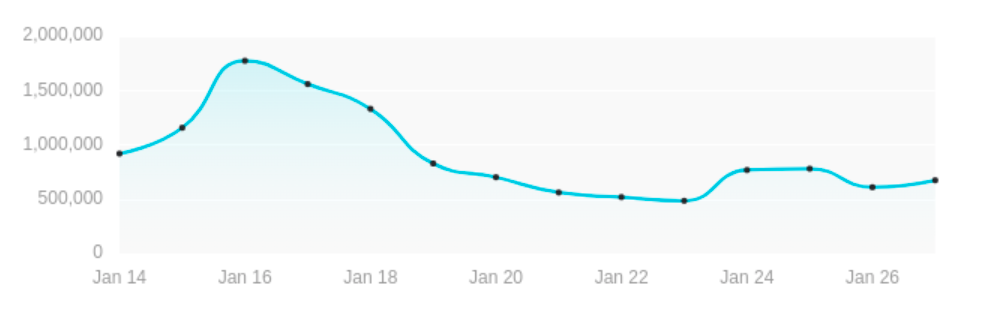
\includegraphics[scale=0.5]{fig/count_of_tr.png}
    \caption{Количество транзакций обработанных в NEAR за последние 14 дней. Дата: 28.01.2022. \url{https://explorer.near.org}} \label{fig:count_of_tr}
\end{figure}

Самая важная концепция NFT - это то, что он дает право доказать, что данный конкретный файл, интеллектуальная собственность, часть данных принадлежит конкретному одному человеку. Если в современном мире права на картину, музыку либо любой другой медиа объект хранятся на каком-нибудь сервере и подкрепляются бумажной подписью на каком-нибудь документе и не без помощи юристов, то NFT позволяет упростить весь этот процесс ненужной бумажной волокиты. Немногие готовы перенести права картины на NFT, но на сегодняшний день есть и примеры, например, блокчейн-компания <<Injective Protocol>> купила картину <<Morons>> художника Бэнкси и сожгла ее в прямом эфире, чтобы в последствии перевести данную картину в NFT\footnote{https://rg.ru/2021/03/04/zachem-sozhgli-kartinu-benksi-za-95-tysiach-dollarov.html}.

Наш маркетплейс строиться на довольно новом блокчейне и будет использоваться непременно как бот, чего я еще не видел. Наверное, такого нет в качестве бота, из-за того, что многие думают, что невозможно предоставить хороший интерфейс для этого, но это совсем неверное представление, ведь Discord API предоставляет невероятный функционал, чтобы пользователю было удобно. Также я не еще не видел такого маркетплейса, где есть хоть какая-нибудь технология связанная с машинным обучением: рекомендация цены за NFT, рекомендации самих NFT, GAN NFT картинок.
             % Введение
\anonsection{Существующие работы и решения}

    На сегодняшний день NFT маркетплейсов огромное количество, на блокчейне Ethereum, как примеры: opensea\footnote{https://opensea.io/}, rarible\footnote{https://rarible.com/}, на Solana: solanart\footnote{https://solanart.io/}. На Near protocol, на данный момент самыми популярными являются: Paras\footnote{https://paras.id/}, Mintbase\footnote{https://www.mintbase.io/}.

    Из двух представленных маркетплейсов, наиболее популярным является Paras. Он представляет базовый функционал маркетплейса: аутентификация в кошелек; покупка, продажа, просмотр NFT. У Paras также есть свой токен - Paras. В Paras представлены следующие медиа файлы: картины, фотографии, пиксель-арты.

    Хоть и Mintbase менее популярен, чем Paras, но представляет гораздо больше видов медиа объектов: 3D модели, gif-изображения, аудио объекты. Но сама подача(оформление сайта) выглядит гораздо хуже, чем в Paras.

    Объединяет данные маркетплейсы то, что у них единый стандарт реализации NFT, предоставленный Near protocol~\cite*{nearspec}. Уже как 3 года есть стандарт ERC-721\footnote{https://ru.bitcoinwiki.org/wiki/ERC-721}, который был утвержден сообществом Ethereum. Стандарт в Near немного расширяет возможности, из-за уникальных возможностей реализованных в Near protocol~\cite*{nearspec}. Наша команда планирует придерживаться данного стандарта и реализовывать его, возможно потребуется некоторое его расширение, но об этом пока неизвестно. Важным вопросом является хранение в блокчейне самого NFT.

    В данном стандарте количество, балансы ограничены 128-битным беззнаковым целочисленным типом. Вся сериализация, десериализация происходит с помощью JSON. Сам контракт отслеживает изменения в хранилище.

    NFT хранит следующую информацию о себе: сам идентификатор токена, ID владельца и метаданные этого токена. Метаданные делятся на типа: первый класс, который хранит версию, название токена, ссылка на информацию, которая представляется в виде JSON, ссылка на sha256 хеш. Другой класс хранит: название, описание, время создания, время истечение представленное в UNIX epoch.

    В Smart-контракте NFT должны быть реализованы следующие функции:
    
    \begin{itemize}
        \item nft\_transfer - <<change operation> функция передачи NFT от одного аккаунта другому.;
        \item nft\_transfer\_call - такая же <<change operation>> функция, что и предыдущая, за исключением того, что вызывается nft\_on\_transfer при удачной передачи NFT и nft\_resolve\_transfer при неудачной попытке;
        \item nft\_token - <<view operation>> функция, которая по ID токена возвращает всю информацию о нем.
    \end{itemize}          % Обзор источников
\section{Smart-контракты}
\label{section.main.smart}

В данной главе будет описываться строение и реализация смарт-контрактов.

\subsection{Структура NFT smart-контракта}
\label{section.main.smart.struct}
В данной подглаве будет описываться строение NFT smart-контракта, написанного на языке Rust. Вся логика соответствует описанному стандарту NEP-171\cite{nftstandart}.
\paragraph{NEAR sdk}
Введем основные функции, структуры, декараторы, которые используются при написании smart-контрактов. Для этого необходим фреймворк near-sdk\cite{nearsdkrs}.

Атрибуты:

\begin{listing}[H]
\begin{minted}[breaklines,fontsize=\scriptsize]{rust}
#[near_bindgen]                                                 /* генерирует smart-контракт, совместимый с блокчейном NEAR */
#[derive(BorshDeserialize, BorshSerialize)]                     /* запоминает состояние контракта */
#[derive(PanicOnDefault)]                                       /* не позволяет инициализировать контракт дефолтными значениями, нужен метод new с декоратором init */
#[payable]                                                      /* помечает метод, который может принимать депозит */
\end{minted}
\caption{Near sdk framework attributes}
\label{near.attributes}
\end{listing}

Структуры:

\begin{listing}[H]
\begin{minted}[breaklines,fontsize=\scriptsize]{rust}
use near_sdk::collections::{LazyOption, LookupMap, UnorderedMap, UnorderedSet};
LookupMap       /* Неитерируемый словарь, который хранит свои значения в боре */
UnorderedMap    /* Итерируемый словарь, который хранит свои значения в боре */
UnorderedSet    /* Итерируемое множество объектов, которые хранятся в боре */
LazyOption      /* Структура, которая лениво инициализируется */
\end{minted}
\caption{Near sdk framework structures}
\label{near.structures}
\end{listing}

Функции:
\begin{listing}[H]
\begin{minted}[breaklines,fontsize=\scriptsize]{rust}
env::storage_byte_cost()            /* стоимость хранения одного байта */
env::attached_deposit()             /* внесенный депозит */
env::predecessor_account_id()       /* предыдущий аккаунт от которого прилетел cross-contract call или это мы сами, если мы первые в цепочке */
env::log_str()                      /* написать лог */
env::prepaid_gas()                  /* количество gas предоставленного для call другой функции */
\end{minted}
\caption{Near sdk framework functions}
\label{near.functions}
\end{listing}

\paragraph{Core Functionality}

Опишем основные структуры и функции\cite{corestandard}, которые используются в NFT контрактах.

\begin{listing}[H]
\begin{minted}[breaklines,fontsize=\scriptsize]{rust}
pub type TokenId = String;

#[derive(BorshDeserialize, BorshSerialize, Serialize, Deserialize, Clone)]
#[serde(crate = "near_sdk::serde")]
pub struct NFTContractMetadata {
    pub spec: String,
    pub name: String,
    pub symbol: String,
    pub icon: Option<String>,
    pub base_uri: Option<String>,
    pub reference: Option<String>,
    pub reference_hash: Option<Base64VecU8>,
}
\end{minted}
\caption{NFT contract metadata}
\label{nftcontract.metadata}
\end{listing}

Структура контракта представляет из себя следующие поля:
\begin{enumerate}
\item spec - версия, является обязательным полем.
\item name - название контракта, является обязательным полем.
\item symbol - краткое название, является обязательным полем.
\item icon - иконка, которая будет отображаться вместе с контрактом(url).
\item base\_uri - url, который ведет на надежное централизованное хранилище данных в reference.
\item reference - url на json с дополнительными данными(json должен располагаться в децентрализованном хранилище).
\item reference\_hash - sha256 хэш от json на который ведет url в поле reference.
\end{enumerate}

\begin{listing}[H]
\begin{minted}[breaklines,fontsize=\scriptsize]{rust}
#[derive(BorshDeserialize, BorshSerialize, Serialize, Deserialize)]
#[serde(crate = "near_sdk::serde")]
pub struct TokenMetadata {
    pub title: Option<String>,
    pub description: Option<String>,
    pub media: Option<String>,
    pub media_hash: Option<Base64VecU8>,
    pub copies: Option<u64>,
    pub issued_at: Option<u64>,
    pub expires_at: Option<u64>,
    pub starts_at: Option<u64>,
    pub updated_at: Option<u64>,
    pub extra: Option<String>,
    pub reference: Option<String>,
    pub reference_hash: Option<Base64VecU8>,
}
\end{minted}
\caption{NFT contract token metadata}
\label{nftcontract.tokenmetadata}
\end{listing}

Структура метаданных токена состоит из следующих полей:
\begin{enumerate}

\item title - название NFT токена.
\item description - описание NFT токена.
\item media - ссылка на содержимое NFT токена, желательно, чтобы эта ссылка вела на децентрализованное хранилище.
\item media\_hash - хэш от содержимого NFT токена, на которое ведет поле media.
\item copies - количество копий NFT токена.
\item issued\_at - время, когда NFT токен был создан.
\item expires\_at - время, когда время жизни NFT токена истекает.
\item starts\_at - время, когда токен начал быть валидным.
\item extra - любые дополнительные данные.
\item reference - ссылка на json с дополнительной информацией о JSON.
\item reference\_hash - sha256 хэш от содержимого на которое ведет ссылка в поле reference.

\end{enumerate}

\begin{listing}[H]
\begin{minted}[breaklines,fontsize=\scriptsize]{rust}
#[derive(BorshDeserialize, BorshSerialize)]
pub struct Token {
    pub owner_id: AccountId,
    pub next_approval_id: u64,
    pub approved_account_ids: HashMap<AccountId, u64>,
    pub royalty: HashMap<AccountId, u32>
}

#[derive(Serialize, Deserialize)]
#[serde(crate = "near_sdk::serde")]
pub struct JsonToken {
    pub token_id: TokenId,
    pub owner_id: AccountId,
    pub metadata: TokenMetadata,
    pub approved_account_ids: HashMap<AccountId, u64>,
    pub royalty: HashMap<AccountId, u32>
}
\end{minted}
\caption{NFT contract token structs}
\label{nftcontract.tokenstructs}
\end{listing}

Структура NFT токена представляет из себя 3 связанные структуры:
\begin{enumerate}
    \item TokenMetadata - метаданные токена, где каждое из полей является опциональным.
    \item Token - для каждого токена образуется связь:
    \begin{enumerate}
        \item owner\_id - аккаунт владельца токена.
        \item approved\_accounts\_ids - словарь из доверенных аккаунтов, где значения является счетчик версий.
        \item next\_approval\_id - текущая версия токена.
        \item royalty - доля других аккаунтов, на получение денег с продажи токена.
    \end{enumerate}
    \item JsonToken - endpoint структура, которая возвращается при работе с контрактом извне.
\end{enumerate}

Теперь опишем структуру класса контракта, в котором хранятся созданные токены:
\begin{listing}[H]
\begin{minted}[breaklines,fontsize=\scriptsize]{rust}
#[near_bindgen]
#[derive(BorshDeserialize, BorshSerialize, PanicOnDefault)]
pub struct Contract {
    pub owner_id: AccountId,
    pub tokens_per_owner: LookupMap<AccountId, UnorderedSet<TokenId>>,
    pub tokens_by_id: LookupMap<TokenId, Token>,
    pub token_metadata_by_id: UnorderedMap<TokenId, TokenMetadata>,
    pub metadata: LazyOption<NFTContractMetadata>,
}
\end{minted}
\caption{NFT contract struct}
\label{nftcontract.struct}
\end{listing}

\begin{enumerate}
\item owner\_id - владелец контракта, которые задается единственный раз при инициализации.
\item metadata - метаданные контракта, которые задаются единственный раз при инициализации.
\item tokens\_per\_owner - позволяет по аккаунту получить все токены, которыми владеет.
\item tokens\_by\_id - позволяет по TokenId получить структуру Token описанную выше.
\item tokens\_metadata\_by\_id - позволяет по TokenId получить структуру TokenMetadata описанную выше.
\end{enumerate}

Следующая функция из core functionality без которой нельзя осуществить никакой продажи - создание или mint NFT токена. Функция nft\_mint принимает token\_id, метаданные, владельца и royalties(про них будет рассказано во главе Royalties).
Так как это payable функция, то пользователь должен будет внести депозит для хранения информации о добавляемом токене. Лишний депозит вернется пользователю обратно.
Также в отличие от Paras мы не обязуем пользователя привязывать токен к конкретной коллекции чем с одной стороны дали больше свободы пользавотелю, а с другой стороны упростили реализацию.

Псевдокод будет выглядеть следующим образом (Листинг {\color{blue}\ref{nftcontract.mint}}):

\begin{listing}
\begin{minted}[breaklines,fontsize=\scriptsize]{rust}
#[payable]
fn nft_mint(token_id, metadata, receiver_id, royalties) {
    /* Сохранить начальный storage_usage*/
    start_storage_usage = env::storage_usage();

    /* Распаковать и положить royalties */
    royalty = AcceptRoyalties(royalties);

    /* Создать токен */
    token = CreateToken(metadata, royalties);

    /* Проверить, что такого token_id не существует */
    assert(!Exist(token_id));

    /* Добавить токен в необходимые структуры */
    contract.tokens_by_id.Insert(token_id, token);
    contract.token_metadata_by_id.Insert(token_id, metadata);
    add_token_to_owner(token.owner_id, token_id);

    /* Вернуть неиспользованный депозит */
    refund(env::storage_usage() - start_storage_usage);
}
\end{minted}
\caption{NFT token mint}
\label{nftcontract.mint}
\end{listing}

Каждый пользователь может запросить на просмотр любой NFT токен с помощью view функции nft\_token, указав в параметрах token\_id.
В качестве результата пользователь получит JsonToken структуру, описанную выше или None, если такого токена не существует (Листинг {\color{blue}\ref{nftcontract.entoken}}).

\begin{listing}
\begin{minted}[breaklines,fontsize=\scriptsize]{rust}
fn nft_token(token_id) -> Option<JsonToken> {
    if !Exist(token_id) {
        return None;
    } else {
        return ConstructJsonToken(token_id);
    }
}
\end{minted}
\caption{NFT nft\_token}
\label{nftcontract.entoken}
\end{listing}

Последние функции из core functionality отвечают за передачу nft токена:
\begin{enumerate}
\item nft\_transfer - отправить токен другому аккаунту.
\item nft\_transfer\_call - отправить токен другому аккаунту для выполнения какой-то услуги, то есть должна будет выполниться какая-то дополнительная логика на другом smart-контракте.
\item nft\_on\_transfer - дополнительная логика, которая должна исполниться в другом контракте после nft\_transfer\_call.
\item nft\_resolve\_transfer - функция, которая определяет нужно ли возвращать токен обратно или нет после nft\_on\_transfer.
\end{enumerate}
С первой функция все ясно, она просто отправляет токен, а со второй лучше привести иллюстрацию:

\begin{figure}[H]
	\centering
	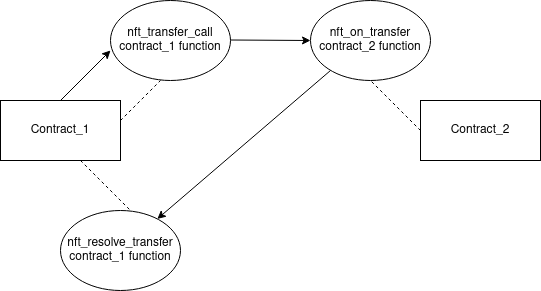
\includegraphics[height=70mm]{fig/temp.png}
	\caption{nft\_transfer\_call}
\end{figure}

Смоделируем пример, где мы хотим отправить из contract\_1 свой токен в другой контракт contract\_2 и выполнить в нем дополнительную сервисную логику(например contract\_2 это контракт маркетплейса, который должен будет выставить что-то на продажу).
Тогда сервисная логика должна будет реализована в nft\_on\_transfer. Вызывать ее должен будет nft\_transfer\_call и завершать всю эту цепочку должна будет функция nft\_resolve\_transfer.
Псевдокод функций будет выглядеть следующим образом(Листинг {\color{blue}\ref{nftcontract.transfer1}}):

\begin{listing}
\begin{minted}[breaklines,fontsize=\scriptsize]{rust}
fn nft_on_transfer(sender_id, previous_owner_id, token_id, msg) -> Promise;

#[payable]
fn nft_transfer_call(receiver_id, token_id, approval_id, msg) -> PromiseOrValue<bool> {

    /* Сохраняем отправителя и копию токена до отправки */
    sender_id = env::predecessor_account_id();
    previous_token = own_contract.internal_transfer(sender_id, receiver_id, token_id, approval_id);

    /* Если отправитель не владелец, значит мы ему доверили наш токен, подробнее в главе approval managements */
    authorized_id = None;
    if sender_id != previous_token.owner_id {
        authorized_id = sender_id;
    }

    /* Вызываем nft_on_transfer на другом контракте, потом nft_resolve_transfer на своем */
    return reciever_contract::nft_on_transfer(
        sender_id,
        previous_token.owner_id,
        token_id,
        msg,
        receiver_id,
    ).then(
        own_contract::nft_resolve_transfer(
            authorized_id,
            previous_token.owner_id,
            receiver_id,
            token_id,
            previous_token.approved_account_ids,
        )
    )
}

#[private]
fn nft_resolve_transfer(
    authorized_id,
    owner_id, receiver_id,
    token_id, approved_account_ids,
) -> bool {

    /* Передача произошла успешно */
    if IsSuccesfull() {
        return true
    }

    /* Иначе возвращаем токен обратно владельцу */
    own_contract.internal_remove_token_from_owner(receiver_id, token_id);
    own_contract.internal_add_token_to_owner(owner_id, token_id);
    token.owner_id = owner_id;
    refund_approved_account_ids(receiver_id, token.approved_account_ids);
    token.approved_account_ids = approved_account_ids;
    own_contract.tokens_by_id.insert(token_id, token);

    return false
}
\end{minted}
\caption{NFT contract transfer}
\label{nftcontract.transfer1}
\end{listing}

\paragraph{Enumeration}
Для удобного взаимодействия с контрактом, необходимо добавить больше view функций с pagination для просмотра NFT токенов\cite{enumstandard}:
\begin{enumerate}
\item nft\_total\_supply - получить общее количество существующих токенов.
\item nft\_tokens - получить существующие токены, используя pagination.
\item nft\_supply\_for\_owner - получить общее количество существующих токенов для конкретного аккаунта.
\item nft\_token\_for\_owner - получить существующие токены для конкретного аккаунта, используя pagination.
\end{enumerate}

Псевдокод будет выглядеть следующим образом(Листинг {\color{blue}\ref{nftcontract.transfer}}):

\begin{listing}
\begin{minted}[breaklines,fontsize=\scriptsize]{rust}
pub fn nft_total_supply() -> U128 {
    return length(own_contract.token_metadata_by_id)
}

pub fn nft_tokens(from_index, limit) -> Vec<JsonToken> {
    return own_contract.token_metadata_by_id.keys()
        .skip(from_index)
        .take(limit)
        .map(|token_id| self.nft_token(token_id))
        .collect()
}

pub fn nft_supply_for_owner(account_id) -> U128 {
    if Exist(account_id) {
        return length(own_contract.tokens_per_owner.get(account_id))
    } else {
        return 0
    }
}

pub fn nft_tokens_for_owner(
    account_id,
    from_index,
    limit
) -> Vec<JsonToken> {
    if Exist(account_id) {
        return tokens.iter()
            .skip(from_index)
            .take(limit)
            .map(|token_id| self.nft_token(token_id))
            .collect()
    } else {
        return vec![];
    }
}
\end{minted}
\caption{NFT contract enumeration}
\label{nftcontract.transfer}
\end{listing}

\paragraph{Approval Management}
Необходимо добавить функционал передачи своего токена другим аккаунтом от своего имени\cite{approvalstandard}. Для этого будет хранить список доверенных аккаунтов(approved\_account\_ids).
Также структура токена хранит next\_approval\_id, который изначально равен 0 и увеличивается на единицу при каждом новом добавленном доверенном аккаунте.

Рассмотрим пример, где account\_1 решил создать токен, тогда у него будет следующая структура(Листинг {\color{blue}\ref{nftcontract.approval1}}):
\begin{listing}
\begin{minted}[breaklines,fontsize=\scriptsize]{rust}
Token: {
    owner_id: account_1
    approved_accounts_ids: {}
    next_approval_id: 0
}
\end{minted}
\caption{NFT contract approval management}
\label{nftcontract.approval1}
\end{listing}

Если он решит добавить account\_2, account\_3, как доверенные тогда структура станет следующей(Листинг {\color{blue}\ref{nftcontract.approval2}}):
\begin{listing}[H]
\begin{minted}[breaklines,fontsize=\scriptsize]{rust}
Token: {
    owner_id: account_1
    approved_accounts_ids: {
        account_2: 0,
        account_3: 1
    }
    next_approval_id: 2
}
\end{minted}
\caption{NFT contract approval management}
\label{nftcontract.approval2}
\end{listing}

Счетчик next\_approval\_id  необходим, чтобы не случилось случая, когда новый владелец токена решил добавить доверенный аккаунт, который был до этого. Такие случаи могут испортить всю логику на других smart-контрактах.
Подробнее краевые случаи описаны в стандарте\cite{approvalstandard}.

Approval Management не добавляет новых внешних view функций или payable функций, а просто вносит некоторую дополнительную логику проверки в существующие функции из секции Core Functionality.

\paragraph{Royalties}

Последнее чего требует стандарт - распределение прибыли от продажи NFT или от любой другой логики, которая будет возвращать NEAR среди нескольких аккаунтов в зависимости от долей\cite{royaltystandard}.
Для этого у нас есть поле royalty в структуре Token, которая отображает пары в соответствующие доли. Сумма всех долей должна быть равна 10.000.

Также добавятся две новые функции:
\begin{enumerate}
\item nft\_payout - получить распределение баланса в зависимости от долей для конкретного token\_id.
\item nft\_transfer\_payout - совершить перевод токена и вернуть распределение баланса от долей.
\end{enumerate}
Псевдокод будет выглядеть следующим образом(Листинги  {\color{blue}\ref{nftcontract.approval3}} и {\color{blue}\ref{nftcontract.approval4}}):
\begin{listing}
\begin{minted}[breaklines,fontsize=\scriptsize]{rust}
fn nft_payout(token_id, balance) -> Payout {
    /* Проверить, что токен существует */
    assert(ExistToken(token_id))

    /* Достать структуру токен */
    token = own_contract.tokens_by_id.get(token_id);
    result = PayoutConstruct();

    /* Посчитать доли других аккаунтов */
    current_sum = 0;
    for (key, value) in Iter(token.royalty) {
        if key == token.owner_id {
            continue;
        }
        result.payout.insert(
            key, CalcPayout(value, balance)
        );
        current_sum += value;
    }
    /* Посчитать свою долю */
    result.payout.insert(token.owner_id, CalcPayout(10000 - current_sum, balance));
    return result
}
\end{minted}
\caption{NFT contract nft\_payout}
\label{nftcontract.approval3}
\end{listing}

\begin{listing}
\begin{minted}[breaklines,fontsize=\scriptsize]{rust}
#[payable]
fn nft_transfer_payout(
    receiver_id, token_id,
    approval_id, balance,
) -> Payout {
    /* Отправить токен */
    sender_id = env::predecessor_account_id();
    prev_token = own_contract.internal_transfer(sender_id, receiver_id, token_id, approval_id);

    result = PayoutConstruct();

    /* Посчитать доли других аккаунтов */
    current_sum = 0;
    for (key, value) in Iter(prev_token.royalty) {
        if key == prev_token.owner_id {
            continue;
        }
        result.payout.insert(key, CalcPayout(value, balance));
        current_sum += value;
    }
    /* Посчитать свою долю */
    result.payout.insert(prev_token.owner_id, CalcPayout(10000 - current_sum, balance));
    return result
}
\end{minted}
\caption{NFT contract nft\_transfer\_payout}
\label{nftcontract.approval4}
\end{listing}

\subsection{Структура маркетплейс smart-контракта}

В данной главе будет описано строение маркетплейс smart-контракта. Контракт маркетплейса уже не подчиняется никакому стандарту и может быть реализован разными способами.

\paragraph{Core functionality}

Начнем с функций, которые должны быть доступны пользователю:
\begin{enumerate}
    \item Выставить NFT токен на продажу.
    \item Обновить цену своего выставленного на продажу NFT токена.
    \item Убрать с продажи свой выставленный до этого NFT токен.
    \item Получить список выставленных на продажу NFT токенов.
    \item Купить выставленный на продажу NFT токен.
\end{enumerate}

Заметим, что на маркетплейс должны уметь выставлять токены нескольких NFT контрактов, потому что все они стандартизированны.
То есть пользователи могут покупать/продавать токены абсолютно разных NFT контрактов.

\begin{figure}[h!]
	\centering
	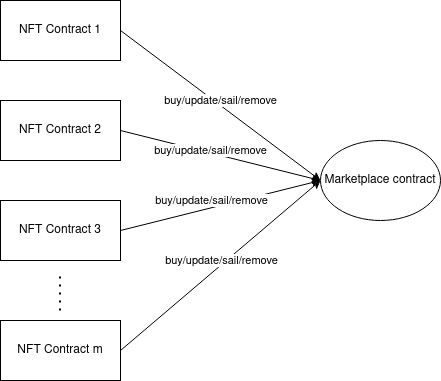
\includegraphics[height=70mm]{fig/marketplace.png}
	\caption{Marketplace core functionality}
\end{figure}

Опишем структуру маркетплейс контракта(Листинг {\color{blue}\ref{marketplacecontract.struct}}):

\begin{listing}
\begin{minted}[breaklines,fontsize=\scriptsize]{rust}

/* Так как выставить токен могут с разных контрактов, удобно будет соединить их в одной строке */
/* ContractAndTokenId = contract ID + DELIMITER + token ID */
pub type ContractAndTokenId = String;
/* Цена токенов будет в YoctoNear */
pub type SalePriceInYoctoNear = U128;
pub type TokenId = String;

/* Структура NFT токена выставленного на продажу */
#[derive(BorshDeserialize, BorshSerialize, Serialize, Deserialize)]
#[serde(crate = "near_sdk::serde")]
pub struct Sale {
    /* Владелец NFT токена */
    pub owner_id: AccountId,

    /* Значение этого поля обоснован в главе Approval Management */
    pub approval_id: u64,

    /* nft_contract_id с которого был выставлен NFT токен */
    pub nft_contract_id: String,

    /* Идентификатор выставленного токена */
    pub token_id: String,

    /* Цена */
    pub sale_conditions: SalePriceInYoctoNear,
}

/* Структура контракта */
#[near_bindgen]
#[derive(BorshDeserialize, BorshSerialize, PanicOnDefault)]
pub struct Contract {
    /* Владелец контракта */
    pub owner_id: AccountId,

    /* Выставленные на продажу токены по ContractAndTokenId */
    pub sales: UnorderedMap<ContractAndTokenId, Sale>,

    /* Выставленные на продажу ContractAndTokenId по конкретному аккаунту */
    pub by_owner_id: LookupMap<AccountId, UnorderedSet<ContractAndTokenId>>,

    /* Выставленные на продажу токены по конкретному аккаунту */
    pub by_nft_contract_id: LookupMap<AccountId, UnorderedSet<TokenId>>,

    /* Внесенная сумма на хранение nft токена */
    /* Смысл данной структуры будет обоснован позже */
    pub storage_deposits: LookupMap<AccountId, Balance>,
}
\end{minted}
\caption{Marketplace contract struct}
\label{marketplacecontract.struct}
\end{listing}

Когда пользователь хочет выставить на продажу NFT токен, он должен вызвать nft\_approve у своего NFT контракта, чтобы добавить аккаунт маркетплейса в доверенные аккаунты, тогда на контракте маркетплейса вызовется метод nft\_on\_approve, который добавит токен на продажу.
В результате, когда другой пользователь захочет купить токен, то маркетплейс сможет легко перевести его новому владельцу, потому он является доверенным аккаунтом для продаваемого токена.

На иллюстрации будет приведен пример, где пользователь выставляет на продажу два токена с двух разных NFT контрактов на одном маркетплейс контракте.

\begin{figure}[H]
	\centering
	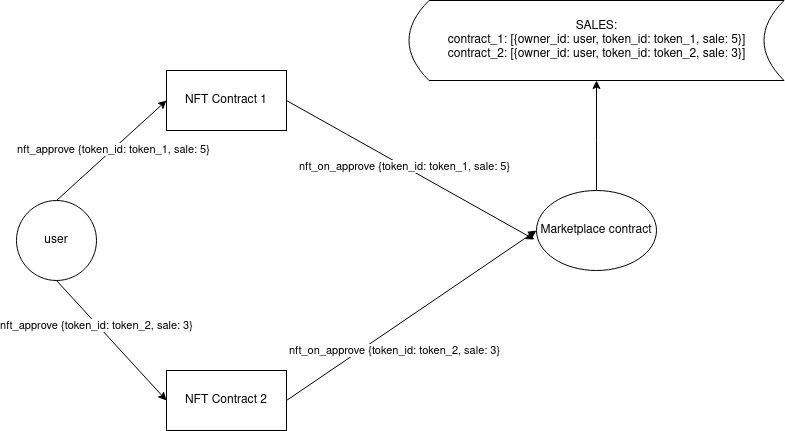
\includegraphics[height=70mm]{fig/sell.png}
	\caption{Marketplace contract sell}
\end{figure}

Псевдокод будет выглядеть следующим образом:(Листинг {\color{blue}\ref{marketplacecontract.onapprove}})

\begin{listing}
\begin{minted}[breaklines,fontsize=\scriptsize]{rust}
fn nft_on_approve(token_id, owner_id, approval_id, sale_price) {
    /* NFT контракт с которого был вызвана продажа */
    nft_contract_id = env::predecessor_account_id();

    /* Аккаунт пользователя, который подписал контракт */
    signer_id = env::signer_account_id();

    assert(owner_id == signer_id)

    /* Считаем сколько нужно на хранилище и сколько внесено */
    paid_storage = own_contract.storage_deposits.getPaidStorage(signer_id);
    required_storage = CalcRequiredStorage();
    assert(paid_storage > required_storage);

    /* Добавляем покупку в необходимые структуры */
    contract_and_token_id = nft_contract_id + '.' + token_id;
    own_contract.sales.InsertNewSale(
        contract_and_token_id, owner_id, approval_id, nft_contract_id, token_id, sale_price
    );

    own_contract.by_owner_id.InsertNewSale(
        contract_and_token_id, owner_id, approval_id, nft_contract_id, token_id, sale_price
    );

    own_contract.by_nft_contract_id.InsertNewSale(
        owner_id, approval_id, nft_contract_id, token_id, sale_price
    );
}
\end{minted}
\caption{Marketplace contract nft\_on\_approve}
\label{marketplacecontract.onapprove}
\end{listing}

Так как мы делаем cross-contract call между двумя контрактами, тогда определить необходимые средства на хранения продаваемого NFT токена выглядит проблематичным.
Поэтому пользователь должен будет сам покупать хранилище и сам его освобождать, когда его токены продались и место освободилось. Именно для этого необходимо поле storage\_deposits в контракте.
Для внесения near под хранение используется функция storage\_deposit, а для вывода near за неиспользуемое место storage\_withdraw. Логика их кажется тривиальной, поэтому псевдокод приводиться не будет.

Изменение цены и отмена продажи, тоже выглядят достаточно тривиальными, напишем короткий псевдокод(Листинг {\color{blue}\ref{marketplacecontract.update}}):

\begin{listing}
\begin{minted}[breaklines,fontsize=\scriptsize]{rust}
#[payable]
pub fn remove_sale(nft_contract_id, token_id) {
    /* Проверим, что владелец токена пытается его убрать с продажи */
    assert (own_contract.sales.OwnerByToken(token_id) == env::precessor_account_id());

    /* Удаляем продажу из структур контракта */
    contract_and_token_id = nft_contract_id + '.' + token_id;
    own_contract.sales.RemoveByToken(token_id);
    own_contract.by_owner_id.RemoveByContractAndToken(owner_id, contract_and_token_id);
    own_contract.by_nft_contract_id.RemoveByContractAndToken(contract_and_token_id, token_id);
}

#[payable]
pub fn update_price(nft_contract_id, token_id, price) {
    /* Проверим, что владелец токена пытается его убрать с продажи */
    assert (self.sales.OwnerByToken(token_id) == env::precessor_account_id());

    /* Обновим цену продажи в структурах контракта */
    contract_and_token_id = nft_contract_id + '.' + token_id;
    own_contract.sales.UpdateByToken(token_id, price);
}
\end{minted}
\caption{Marketplace contract update price/remove sale}
\label{marketplacecontract.update}
\end{listing}

Покупка осуществляется следующим образом: пользователь дергает nft\_offer команду у маркетплейс контракта, тот в свою очередь вызывает nft\_transfer\_payout на NFT контракте, а потом завершает или отменяет покупку используя resolve\_purchase.
Функция resolve\_purchase при удачной покупке разделит сумму продажи относительно долей royalties. Данные величины нам возвращает функция nft\_transfer\_payout.

Схема покупки выглядит следующим образом(рис. {\color{blue}\ref{marketplacecontract.buypng}}), а с псевдокодом функций покупки можно ознакомиться в Листинге {\color{blue}\ref{marketplacecontract.buy}}:

\begin{listing}
\begin{minted}[breaklines,fontsize=\scriptsize]{rust}
#[payable]
pub fn offer(nft_contract_id, token_id) {
    /* Смотрим сколько пользователь внес депозита */
    deposit = env::attached_deposit();

    contract_token_id: String = contract_id + '.' + token_id;
    
    /* Получаем структуру продажи для token_id из нужного NFT контракта */
    offer_sale = own_contract.sales.get(contract_token_id);
    buyer_id = env::predecessor_account_id();
   
    /* Проверяем, что внесенный депозит больше цены и что покупатель не является владельцем */
    assert(offer_sale.owner_id != buyer_id);
    assert(deposit >= offer_sale.sale_conditions);

    own_contract.process_purchase(contract_id, token_id, deposit,buyer_id);
}

#[private]
pub fn process_purchase(nft_contract_id, token_id, price, buyer_id) -> Promise {
    /* Удаляем структуру продажи из соответствующих структур */    
    purchased_sale = own_contract.internal_remove_sale(nft_contract_id, token_id);

    /* Вызываем nft_transfer_payout на NFT smart-контракте и завершаем покупку в resolve_purchase */
    nft_contract::nft_transfer_payout(
        buyer_id,
        token_id,
        purchased_sale.approval_id,
        price
    ).then(own_contract::resolve_purchase(
        buyer_id,
        price
    ))
}

#[private]
pub fn resolve_purchase(
    buyer_id,
    price,
) -> U128 {
    /* Если операция nft_transfer_payout на контракте NFT была выполнена успешно */    
    if IsSuccess() {
        /* Получаем payout структуру из nft_transfer_payout */
        payout = PromisResult();

        /* Отправляем каждому royalti аккаунту соответствующую долю */ 
        for (receiver_id, amount) in payout {
            Transfer(receiver_id, amount);
        }
        return price;
    } else {
        return None;
    }
}
\end{minted}
\caption{Marketplace contract buy}
\label{marketplacecontract.buy}
\end{listing}

\begin{figure}[h]
	\centering
	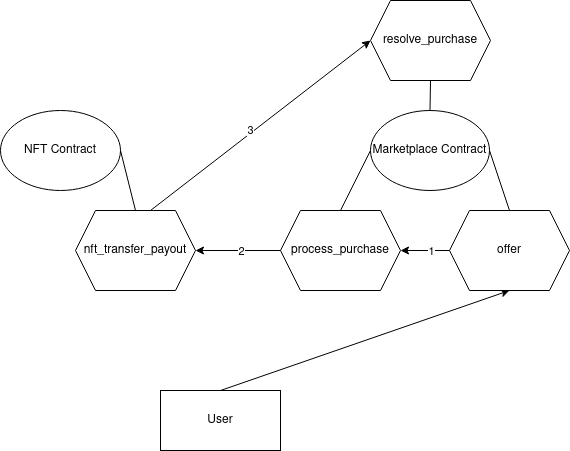
\includegraphics[height=70mm]{fig/buy.png}
	\caption{Marketplace contract buy}
    \label{marketplacecontract.buypng}
\end{figure}

\paragraph{Enumeration}

Для того чтобы удобно взаимодействовать с маркетплейс контрактом были добавлены несколько view функций, которые позволяют выгружать продаваемые NFT.
\begin{enumerate}
\item get\_supply\_sales - получить суммарное количество выставленных токенов.
\item get\_supply\_by\_owner\_id - получить суммарное количество выставленных токенов за определенным пользователем.
\item get\_supply\_by\_nft\_contract\_id - получить суммарное количество выставленных токенов за определенным NFT контрактом.
\item get\_sales\_by\_nft\_contract\_id - получить выставленные на продажу токены за определенным NFT контрактом, используя pagination.
\item get\_sales\_by\_owner\_id - получить выставленные на продажу токены за определенным пользователем, используя pagination.
\item get\_sale - получить определенный продаваемый токен.
\end{enumerate}

Псевдокод данных функций будет выглядеть следующим образом(Листинг {\color{blue}\ref{marketplacecontract.enumeration}}):

\begin{listing}
\begin{minted}[breaklines,fontsize=\scriptsize]{rust}
pub fn get_supply_sales() -> u64 {
    return length(own_contract.sales);
}

pub fn get_supply_by_owner_id(account_id) -> u64 {
    owner_id = own_contract.by_owner_id.get(account_id);
    return length(owner_id);
}

pub fn get_sales_by_owner_id(account_id, from_index, limit) -> Vec<Sale> {
    sales = owner_contract.by_owner_id.get(account_id);

    sales.iter()
        .skip(from_index)
        .take(limit)
        .map(|token_id| owner_contract.sales.get(token_id))
        .collect()
}

pub fn get_supply_by_nft_contract_id(nft_contract_id) -> u64 {
    nft_contract_id = own_contract.by_nft_contract_id.get(nft_contract_id);
    return length(nft_contract_id);
}

pub fn get_sales_by_nft_contract_id(nft_contract_id, from_index, limit) -> Vec<Sale> {
    let sales = own_contract.by_nft_contract_id.get(nft_contract_id);

    sales.iter()
        .skip(from_index)
        .take(limit)
        .map(|token_id| own_contract.sales.get(nft_contract_id, '.', token_id))
        .collect()
}

pub fn get_sale(nft_contract_token) -> Option<Sale> {
    own_contract.sales.get(nft_contract_token)
}
\end{minted}
\caption{Marketplace contract enumeration}
\label{marketplacecontract.enumeration}
\end{listing}

\section{Discord-бот}
\label{section.main.bot}

\subsection{Взаимодействие с блокчейнами}

В данной главе описано ядровое устройство discord-бота: описание работы near-api-js и его переписывание под устройство Discord, устройство метаданных NFT-токена, работа с децентрализованным распределенным хранилищем.

\paragraph{Аккаунты и access keys в NEAR}
Для понимания взаимодействия требуются минимальные знания об аккаунтах и access keys.

Аккаунты в NEAR\cite{nearaccounts} устроены так, что они имеют человеко-читаемый ID в отличие от большинства других блокчейнов, где обычно используется некоторый hash(Рисунок {\color{blue} \ref{fig.eth_near_cmp}}). Длина логина от 2 до 64 символов и содержит в конце суффикс обозначающий сеть блокчейна. Аккаунт может создавать подаккаунты, которые по своему функционалу ничем не отличаются от обычного аккаунта. Данные подаккаунты решают проблему деплоя контрактов: на один аккаунт можно развернуть только один smart-контракт, id аккаунта и будет значить, какой smart-контракт требуется.

\begin{definition}
    В NEAR, как и во всех блокчейнах есть несколько сетей: mainnet, testnet и так далее. Mainnet - главная(продакшн) сеть. Testnet используется для тестирования сервисов.
\end{definition}

Каждый аккаунт имеет создавать множество, которые в NEAR называются access keys. Существует два типа access keys: FullAccess и FunctionCall. Первый дает полный доступ, второй вид ключа уникален и дает разрешения только на подписание функций контрактов. В нашем сервисе не будет использоваться FullAccess access key из-за ненадобности.

\begin{figure}
    \centering
    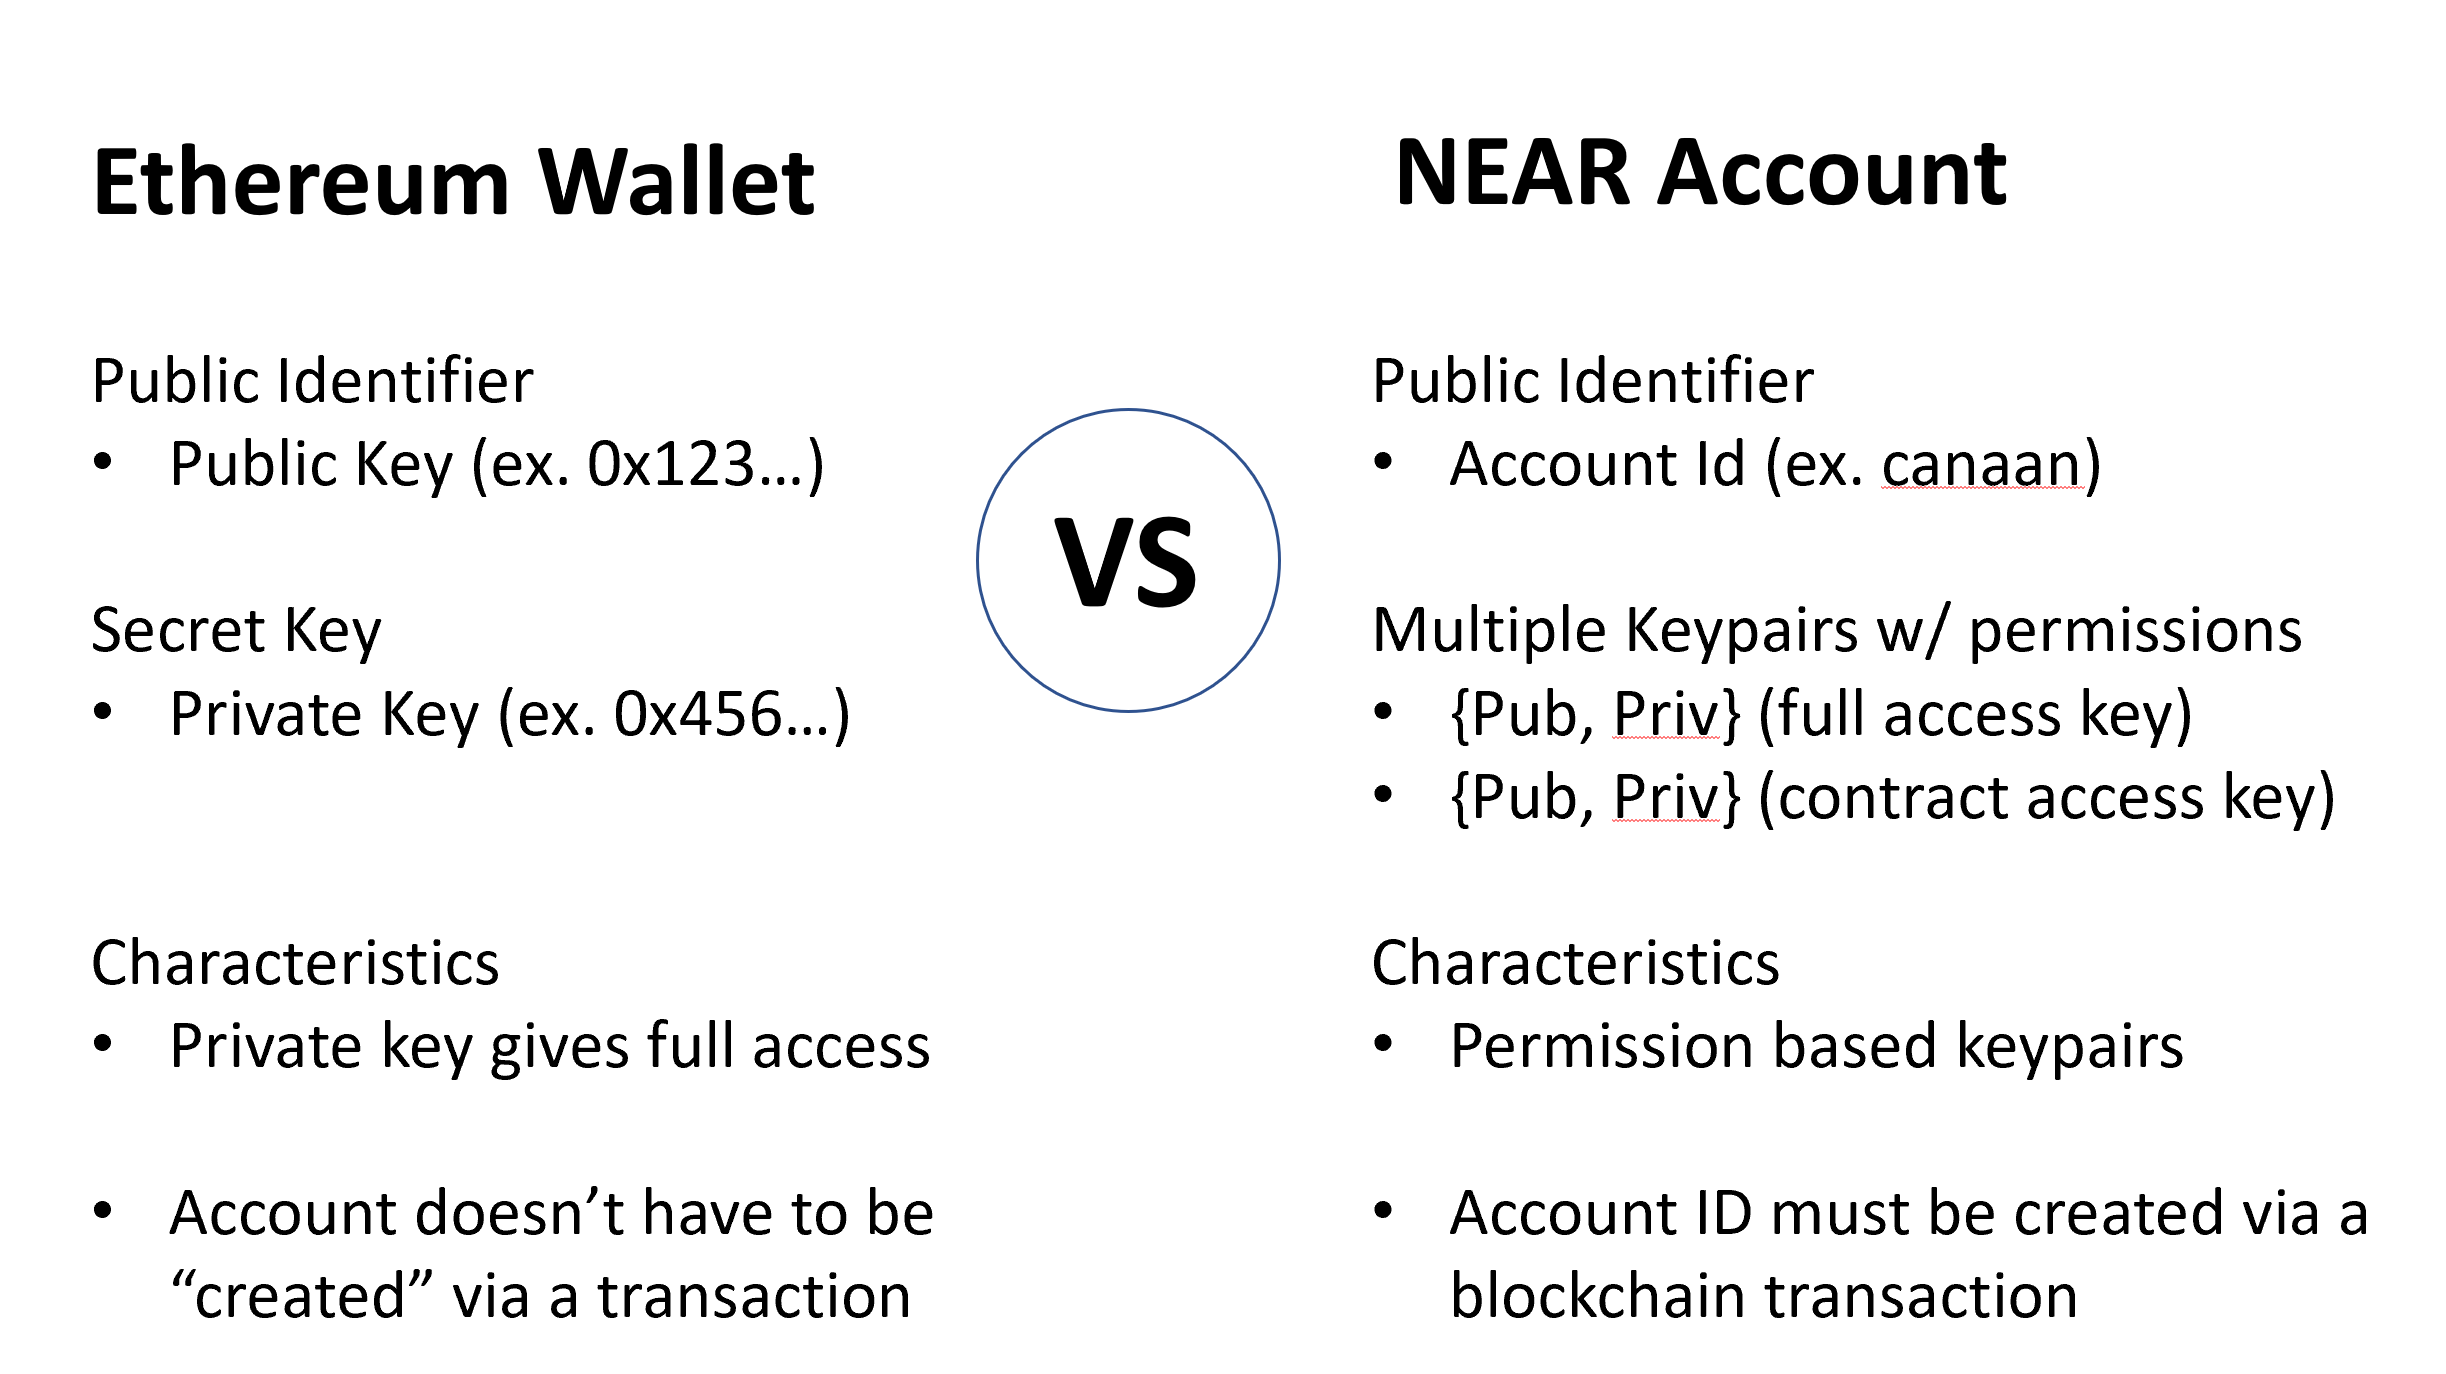
\includegraphics[height=60mm]{fig/eth_near_cmp.png}
    \caption{Сравнение аккаунтов Ethereum и NEAR}
    \label{fig.eth_near_cmp}
\end{figure}

\paragraph{Авторизация в NEAR Wallet}

Авторизация в NEAR Wallet играет роль связывания аккаунта кошелька и пользователя, то есть фактически нам говорит, что у этого пользователя есть этот аккаунт. Наверное, стоит отметить, что, если пользователь авторизовался в NEAR Wallet на нашем сервисе, то от его лица можно вызывать методы контракта, на котором была подписана транзакция(пока не закончатся GAS, которые были указаны при подписании транзакции), к которым не нужно вложение депозита. Данный функционал нам не потребуется, так как у нас либо <<view operations>> в контрактах, либо <<payable change operations>>.

На маркетплейсах в виде сайта вся авторизация происходит на client-side стороне: создается пара ключей(access key) - публичный и секретный; секретный ключ сохраняется в local storage браузера; подписывается транзакция и в последствии этот ключ будет использован сайтом, для подтверждения авторизации(Рисунок {\color{blue} \ref{fig.nearauth.a}}). Сценарий авторизации в discord-бот различается, ведь ключ должен храниться на стороне сервера(Рисунок {\color{blue} \ref{fig.nearauth.b}}). Для этого были необходимо реализовать KeyStore, который взаимодействует с какой-нибудь базой данных на стороне сервера. На роль БД было принято использовать Redis. Был написан KeyStore, который взаимодействует с Redis и функционал, который возвращает URL, а не редеректит пользователя. При любом взаимодействии с ботом, проверяется авторизован ли пользователь, если он не авторизован, то ему предлагается кнопка с URL на подписание транзакции авторизации.

\begin{figure}
	\centering
    \subfloat[Авторизация в NEAR Wallet в near-api-js]{
        \label{fig.nearauth.a}
        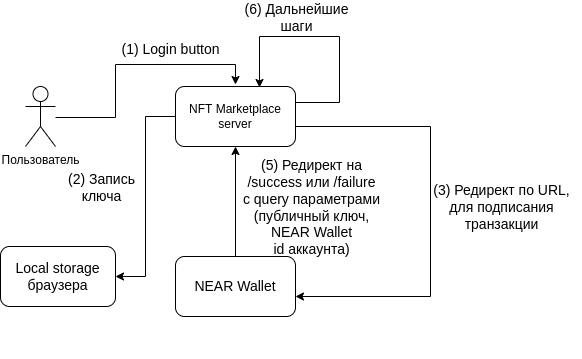
\includegraphics[height=60mm]{fig/auth1.png}
    }
    \subfloat[Авторизация в NEAR Wallet в discord-боте]{
        \label{fig.nearauth.b}
        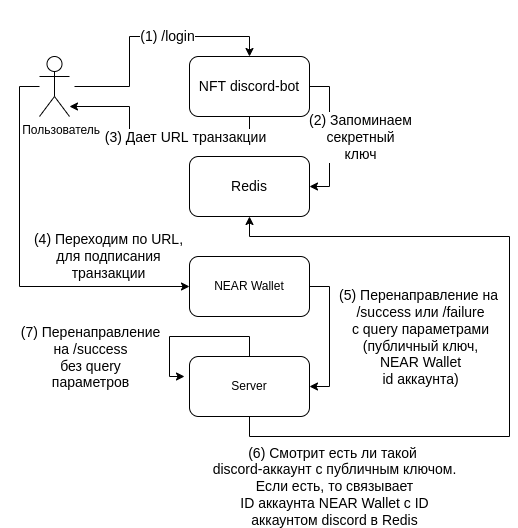
\includegraphics[height=80mm]{fig/auth2.png}
    }
    \caption{}
\end{figure}

\begin{definition}
    Storage --- интерфейс веб API, который позволяет добавлять, изменять, удалять элементы данных, которые представляются в виде ключа и значения\cite{webapistorage}. В веб API есть два объекта, которые используют интерфейс storage: session storage, local storage\cite{webapilocalstorage}. Session storage хранит данные до закрытия браузера, когда как данные в local storage не имеют ограничения по времени и могу быть удалены только намерено.
\end{definition}

\begin{definition}
    KeyStore\cite{nearclasskeystore} --- это класс, который хранит ключи, для подписей транзакций. Их 4 вида: BrowserLocalStorageKeyStore, InMemoryKeyStore, MergeKeyStore, UnencryptedFileSystemKeyStore. BrowserLocalStorageKeyStore пользуется локальным хранилищем браузера для записи, изменения, просмотра значений по ключу. InMemoryKeyStore хранит все в оперативной памяти, используется для тестирования. MergeKeyStore используется для объединения множества KeyStore. UnencryptedFileSystemKeyStore хранит все на диске в виде JSON файла, используется в near cli\cite{nearcli}.
\end{definition}

\paragraph{Вызовы методов у контрактов}

Вызовы методов у smart-контрактов --- это то, чем бот занимается большую часть времени. Как и в случае авторизации, на меркетплейсах в виде сайте подписывание транзакций происходит на client-side стороне(Рисунок {\color{blue} \ref{fig.neartr.a}}): проверка существования access key в local storage браузера, при существовании и еще нескольких условиях идет подписание транзакции без участия пользователя, в ином случае создается URL по которому пользователь подписывает транзакцию. В случае discord-бота(Рисунок {\color{blue} \ref{fig.neartr.b}}) просто выброшена та часть, которую возможно исполнить на client-side стороне и проверка на access key, из-за ненадобности, так как у нас только <<payable change operations>>.

near-api-js не предоставляет хороших оберток для подписания транзакций, в которых несколько Action и Transaction. В нашем случае такие сценарии нужны при отмене продажи NFT и покупки NFT. В случае выставлении на продажу требовалось вызывать методы в таком порядке: <<storage\_deposit>> у контракта маркетплейса для вложения депозита хранения, <<nft\_approve>> у контракта NFT для утверждения маркетплейса в NFT контракте и <<storage\_withdraw>> у контракта маркетплейса для возвращения неиспользуемых NEAR для хранения. В случае отмены продажи: <<offer>> и <<storage\_withdraw>> у контракта маркетплейса. Были написаны данные обертки.

\begin{definition}
    Есть несколько видов Action: CreateAccount, DeployContract, FunctionCall, Transfer, Stake, AddKey, DeleteKey, DeleteAccount. Из этого списка discord-бот использует только FunctionCall, который нужен для вызова методов у smart-контракта. FunctionCall образуется из названия метода, аргументов метода, вносимого депозита и вносимых GAS. Transaction это набор Action, и название контракта, то есть в одном Transaction можно подписывать только методы одного smart-контракта. При подписании транзакции может быть несколько Transaction, что нам позволяет подписывать за раз исполнение разных методов на разных smart-контрактах.
\end{definition}

\begin{figure}
    \centering
    \subfloat[Подпись транзакций в NEAR Wallet в near-api-js]{
        \label{fig.neartr.a}
        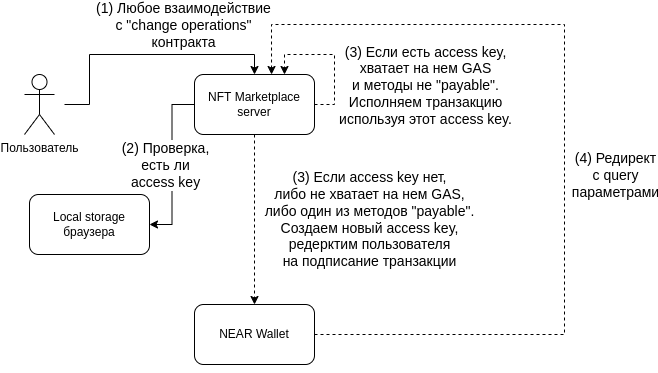
\includegraphics[height=58mm]{fig/transaction1.png}
    }
    \subfloat[Подпись транзакций в NEAR Wallet в discord-боте]{
        \label{fig.neartr.b}
        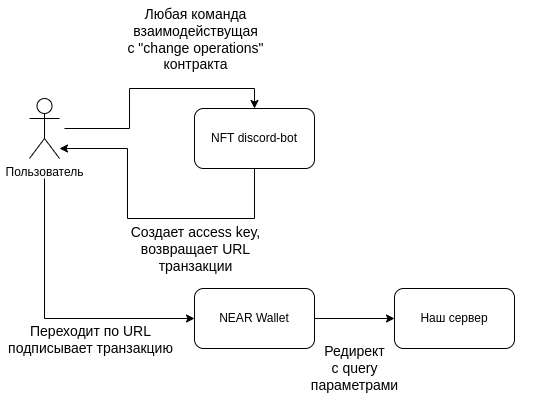
\includegraphics[height=60mm]{fig/transaction2.png}
    }
    \caption{}
\end{figure}

\paragraph{Структура получаемого NFT и его метаданных}
\label{section.main.bot.struct}
На данный момент, при создании NFT в структуре(Листинг {\color{blue}\ref{lst.nftstructure}}) используются следующие поля: <<token\_id>>, <<owner\_id>>, <<royalty>>, <<metadata.title>>, <<metadata.media>>, <<metadata.reference>>. <<metadata.description>> не используется, все описание NFT хранится в метаданных в децентрализованном хранилище в целях экономии оплаты за хранение . В <<metadata.media>>, <<metadata.reference>> хранятся полные URL до медиа-файла и метаданных. В ближайшее время, планируется хранить только CID и только в поле media, так как медиа-файл и метаданные хранятся в одной директории, то для их определения достаточно одного CID(см. {\color{blue} \ref{section.main.bot.storage}}). ID токена при создании формируется следующим образом: ID NEAR аккаунта, который минтит NFT, и текущее время. Такая структура формирования ID токена позволяет искоренить все коллизии.

Структура метаданных(Листинг {\color{blue}\ref{lst.nftmetadata}}) полностью аналогично структуре метаданных в Paras, так как эта структура оправдана своей функциональностью. Только в отличие от Paras нет полей: <<collection>>, <<collection\_id>>, <<blurhash>>, <<mime\_type>>. <<collection>>, <<collection\_id>> нет, потому что на данный момент мы не поддерживаем коллекции NFT. <<mime\_type>>, <<blurhash>> из-за ненадобности.

\begin{listing}
\begin{minted}[breaklines,fontsize=\scriptsize]{js}
{
    token_id: 'chopik.testnet.1652636744470',
    owner_id: 'chopik.testnet',
    approved_account_ids: { 'papamsmarket.pojaleesh.testnet': 2 },
    royalty: { 'chopik.testnet': 10000 },
    metadata: {
        title: 'City',
        description: null,
        media: 'https://bafybeiahhurffoxjubs42l7bl3jjc5zk5vrafiijcxkhex2ukjm3zsbbti.ipfs.dweb.link/f',
        media_hash: null,
        copies: null,
        issued_at: null,
        expires_at: null,
        starts_at: null,
        updated_at: null,
        extra: null,
        reference: 'https://bafybeiahhurffoxjubs42l7bl3jjc5zk5vrafiijcxkhex2ukjm3zsbbti.ipfs.dweb.link/m',
        reference_hash: null
    }
}
\end{minted}
\caption{Структура получаемого NFT}
\label{lst.nftstructure}
\end{listing}

\begin{listing}
\begin{minted}[breaklines,fontsize=\scriptsize]{json}
{
    "description":"Cool city",
    "creator_id":"chopik.testnet",
    "attributes":[
        {"trait_type":"Time","value":"Night"},
        {"trait_type":"Color","value":"Blue"}
    ]
}
\end{minted}
\caption{Структура метаданных NFT в децентрализованном хранилище}
\label{lst.nftmetadata}
\end{listing}

\paragraph{Децентрализованное хранилище данных}
\label{section.main.bot.storage}

Обычно для хранения метаданных и медиа-объекта используется другой блокчейн специализированный под хранение. Связанно это с тем, что при деплое smart-контракта пользователь платит в NEAR за хранение байт, которые хранит контракт, используя механизм, который называется storage staking. На основе storage stacking есть и атаки на smart-контракты, например <<million cheap data additions>> - злоумышленник добавляет огромное количество бесполезных данных при вызове методов, из-за этого в наших контрактах данное обложение в контрактах оплачивает пользователь, которому хочется минимизировать свои растраты на операции. Из-за этого лучше стратегий для хранения объемных файлов(в основном таковыми являются медиа-файлы) это хранить данные в off-chain. Популярным решением является IPFS, при котором любой набор данных представляется удобным адресом - CID. В роли сервиса предоставляющего хранилище был выбран NFT.Storage\cite{nftstorage} --- бесплатное децентрализованное хранилище NFT на IPFS\cite{ipfs} и Filecoin\cite{filecoin}. NFT.Storage предоставляет HTTP API для взаимодействия с хранилищем и обертку на Javascript.

\begin{remark}
    Цена на storage staking устанавливается сетью блокчейна, на данный момент это 1 NEAR за 100 КБ.
\end{remark}

\begin{definition}
    IPFS(InterPlanetary File System) - это протокол распределенной системы обмена файлов. При добавлении файла в IPFS, он делится на маленькие куски, криптографически хэшируется и отдается уникальный фингерпринтр, который называется CID(Content identifier) \cite{ipfs}.
\end{definition}

\begin{remark}
    Для того, чтобы построить стимулирующий слой для сохранения данных в IPFS существует Filecoin. Filecoin - это децентрализованное сетевое хранилище. Filecoin и IPFS - это два разных протокола, взаимодополняющие друг друга. Когда как IPFS позволяет пользователям хранить, запрашивать и передавать друг другу данные, в то время, как Filecoin предназначен для обеспечения системы постоянного хранения.
\end{remark}

\begin{remark}
    Изначально использовался сервис web3storage\cite{web3storage} для хранения, но он отличился медленной загрузкой, получением файлов, из-за чего появилась необходимость в смене на NFT.Storage.
\end{remark}

\subsection{Пользовательский интерфейс}

У пользователя, есть несколько мест откуда он может запускать команды бота: slash-команды(Рисунок {\color{blue} \ref{fig.slashcommands}}), контекстные меню по пользователю(Рисунок {\color{blue} \ref{fig.contextmenu}}) и сами профиля пользователей(Рисунок {\color{blue} \ref{fig.profile}}, Рисунок {\color{blue} \ref{fig.anotherprofile}}). Со своего профиля и с помощью slash-команд, все взаимодействия идут в отношении себя, когда как, при выборе профиля и использовании на нем функционала из контекстного меню операции совершаются в отношении этого пользователя.


\begin{figure}
    \centering
    \subfloat[Slash-команды бота]{
        \label{fig.slashcommands}
        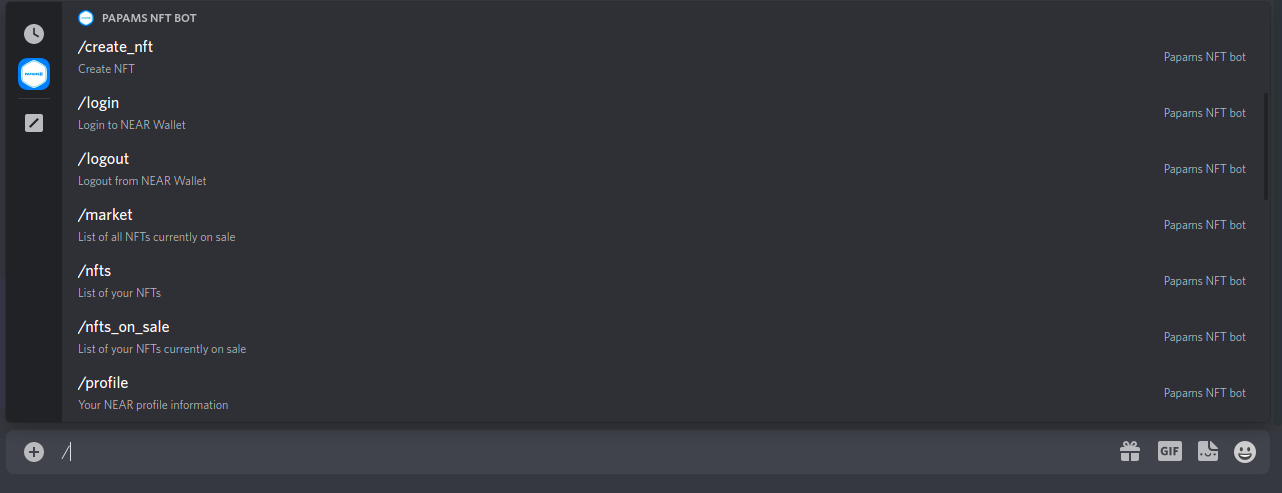
\includegraphics[height=60mm]{fig/slash_commands.png}
    }\\
    \subfloat[Контекстные меню бота]{
        \label{fig.contextmenu}
        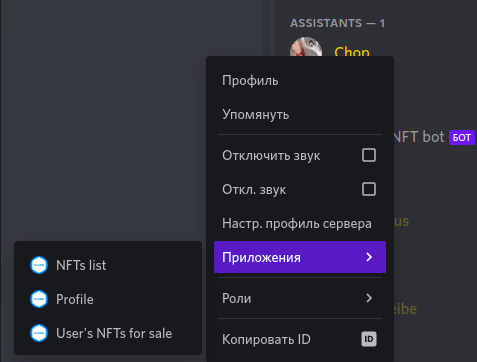
\includegraphics[height=60mm]{fig/context_menu.png}
    }
    \subfloat[Свой профиль пользователя]{
        \label{fig.profile}
        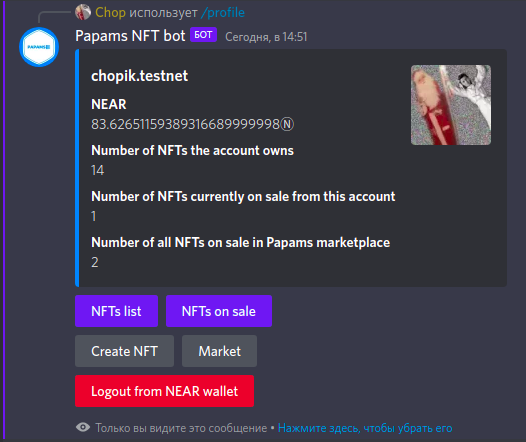
\includegraphics[height=60mm]{fig/profile.png}
    }
    \caption{Точки входа пользователя}
\end{figure}

Авторизация пользователя происходит через соответствующую slash-команду(Рисунок {\color{blue} \ref{fig.authbtn1}}) или при взаимодействии бота в отношении своего профиля, если пользователь не авторизован(Рисунок {\color{blue} \ref{fig.authbtn2}}).

\begin{figure}
    \centering
    \subfloat[Намереная авторизация]{
        \label{fig.authbtn1}
        
\includegraphics[height=30mm]{fig/authbtn1.png}
    }\\
    \subfloat[Предложение об авторизации]{
        \label{fig.authbtn2}
        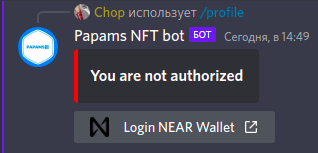
\includegraphics[height=30mm]{fig/authbtn2.png}
    }
    \caption{Авторизация пользователя}
\end{figure}

С помощью контекстных меню(Рисунок {\color{blue} \ref{fig.contextmenu}}), можно взаимодействовать с другими пользователями: мы можем получить профиль пользователя(Рисунок {\color{blue} \ref{fig.anotherprofile}}), его список NFT, список продаваемых NFT(Рисунок {\color{blue} \ref{fig.nftonsaleuser}}).

\begin{remark}
    Если в контекстном меню взаимодействовать с собой, то эффект будет такой-же как от slash-комманд, то есть фактически мы можем не использовать slash-команды вообще и взаимодействовать только через GUI.
\end{remark}

\begin{figure}[H]
    \centering
    \subfloat[Чужой профиль пользователя]{
        \label{fig.anotherprofile}
        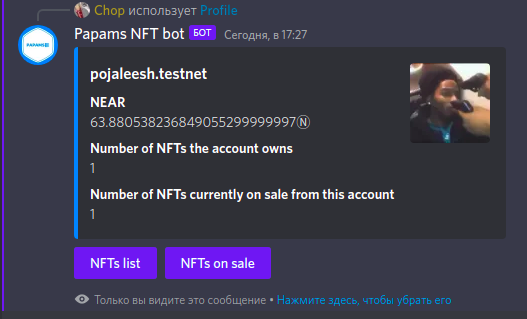
\includegraphics[height=50mm]{fig/anotherprofile.png}
    }
    \subfloat[Взаимодействие с пользователем, если он не авторизован]{
        \label{fig.anotherprofileerror}
        
\includegraphics[height=25mm]{fig/anotherprofileerror.png}
    }
    \caption{Взаимодействия с другими пользователями}
\end{figure}

При взаимодействии с пользователем мы можем купить у него NFT, если таковые имеются(Рисунок {\color{blue} \ref{fig.nftonsaleuser}}). В своем общем списке NFT(Рисунок {\color{blue} \ref{fig.mynftlistonsale}})  или в своем списке продаваемых NFT(Рисунок {\color{blue} \ref{fig.cancelsalenftforsale}}) можно отменить продажу.

\begin{figure}[H]
    \centering
    \subfloat[Список NFT на маркеплейсе]{
        \label{fig.buynftmarket}
        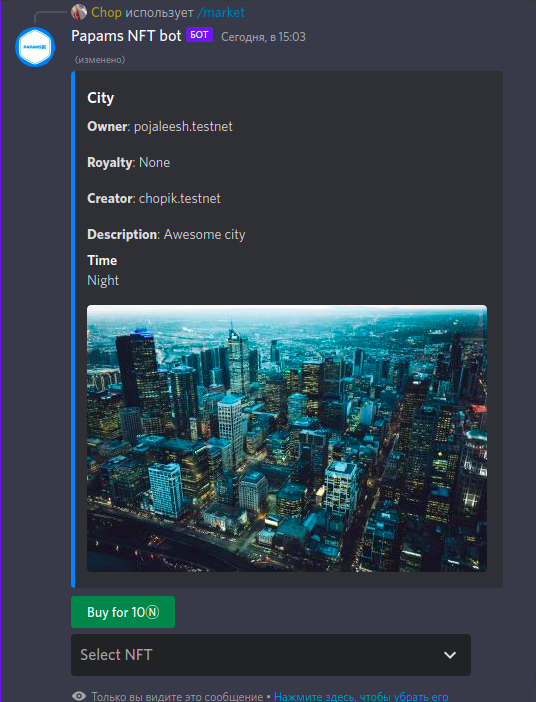
\includegraphics[height=60mm]{fig/buynftmarket.png}
    }
    \subfloat[Список продаваемых NFT у пользователя]{
        \label{fig.nftonsaleuser}
        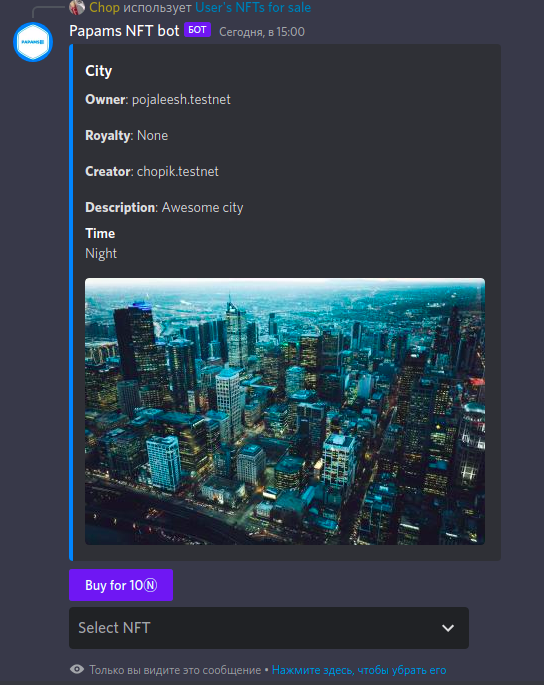
\includegraphics[height=60mm]{fig/nftonsaleuser.png}
    }
    \subfloat[Подтверждение покупки]{
        \label{fig.buyconfirm}
        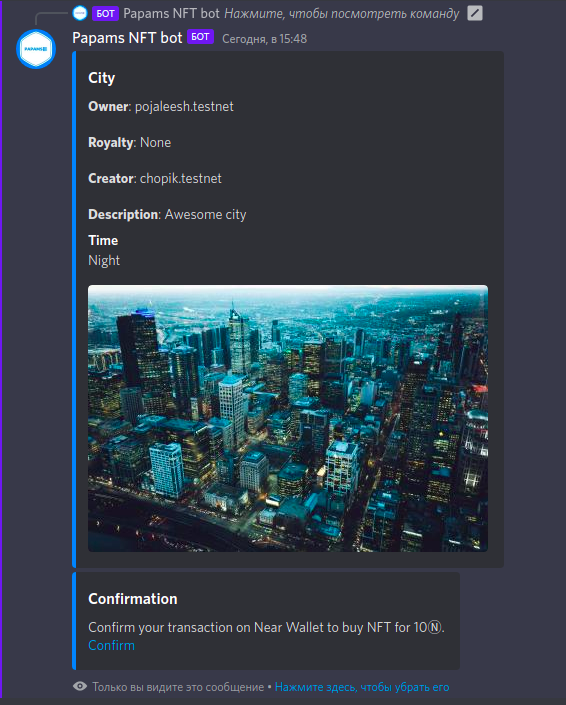
\includegraphics[height=60mm]{fig/buyconfirm.png}
    }
    \caption{Покупка NFT}
\end{figure}

\begin{figure}[H]
    \centering
    \subfloat[Сообщение о переходе в личные сообщения]{
        \label{fig.createnftdm}
        
\includegraphics[height=30mm]{fig/createnftdm.png}
    }\\
    \subfloat[Конструктор NFT]{
        \label{fig.createnftconstructor}
        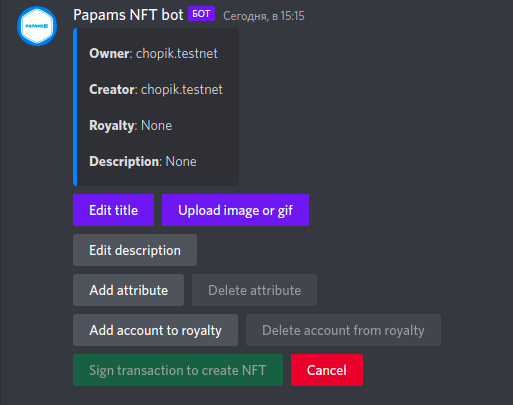
\includegraphics[height=60mm]{fig/createnftconstructor.png}
    }
    \subfloat[Законченное NFT]{
        \label{fig.createnftconstructordone}
        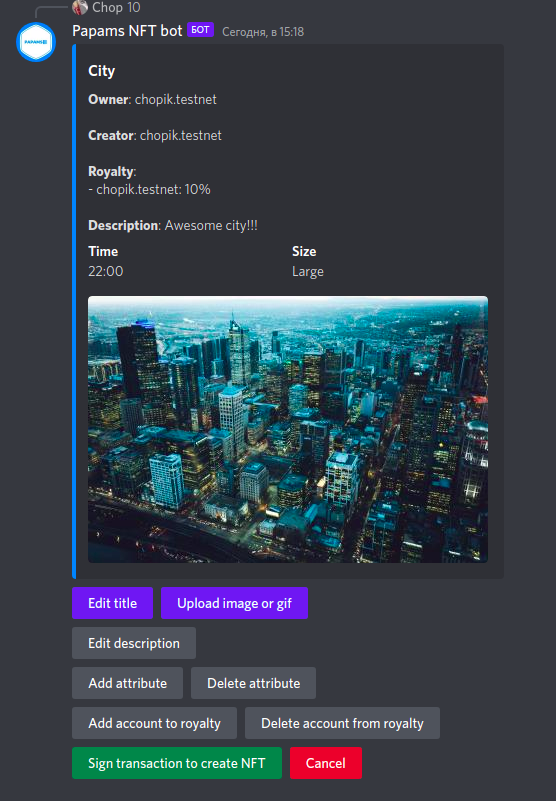
\includegraphics[height=60mm]{fig/createnftconstructordone.png}
    }
    \subfloat[Подтверждение минта]{
        \label{fig.createnftconstructorconfirm}
        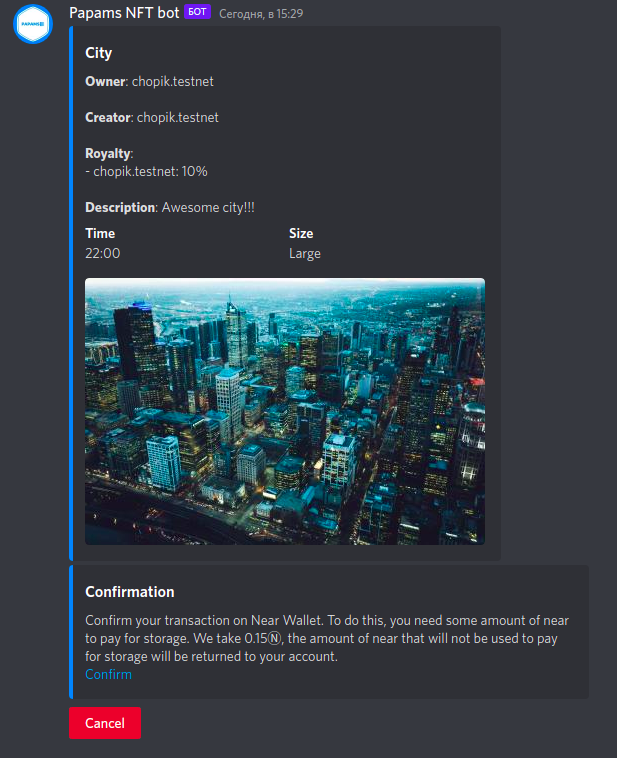
\includegraphics[height=60mm]{fig/createnftconstructorconfirm.png}
    }
    \caption{Минт NFT}
    \label{fig.mintnft}
\end{figure}

Cо своего профиля(Рисунок {\color{blue} \ref{fig.profile}}) или с помощью slash-команды <</create\_nft>> можно запустить процесс создания NFT(Рисунок {\color{blue} \ref{fig.mintnft}}), он переводит пользователя в личные сообщение, так как от пользователя нужен будет медиа-объект, для загрузки которого, пока что нет функционала не через сообщения. NFT собирается в виде конструктора: NFT строится при добавлении нового элемента.

\begin{figure}
    \centering
    \subfloat[Список пользователя со всеми NFT]{
        \label{fig.mynftlistcansale}
        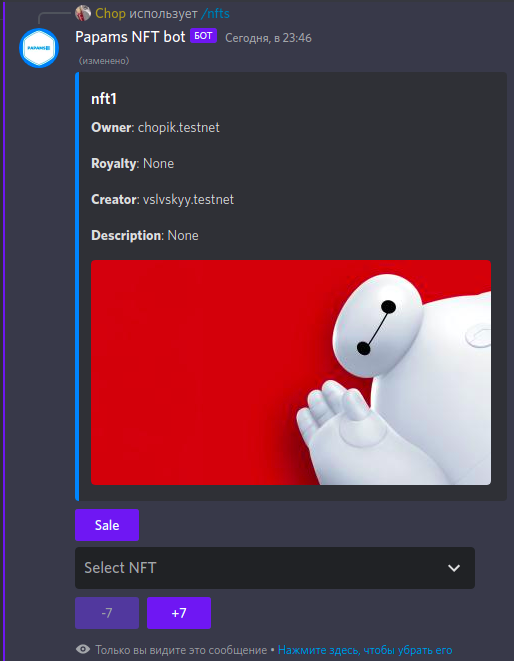
\includegraphics[height=60mm]{fig/mynftlistcansale.png}
    }
    \subfloat[Подтверждение продажи]{
        \label{fig.saleconfirm}
        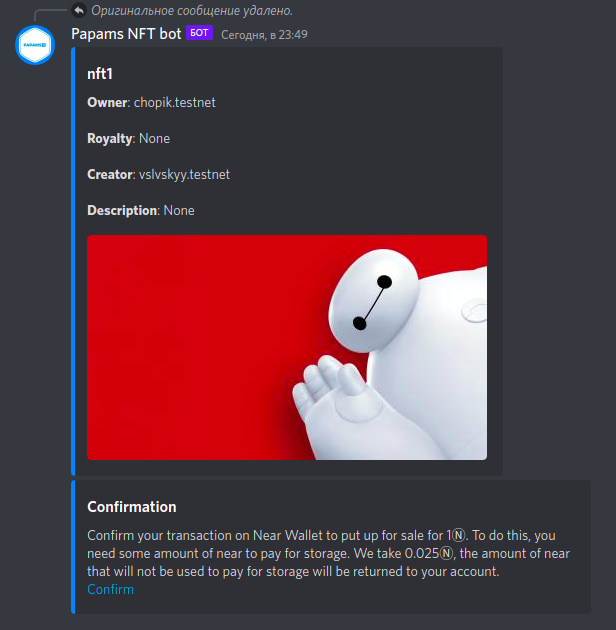
\includegraphics[height=60mm]{fig/saleconfirm.png}
    }
    \caption{Выставление NFT на продажу // Тут еще будет скрин с модалом, когда я переделаю установку цены на модалы}
\end{figure}

\begin{figure}[H]
    \centering
    \subfloat[Список продаваемых пользователем NFT]{
        \label{fig.cancelsalenftforsale}
        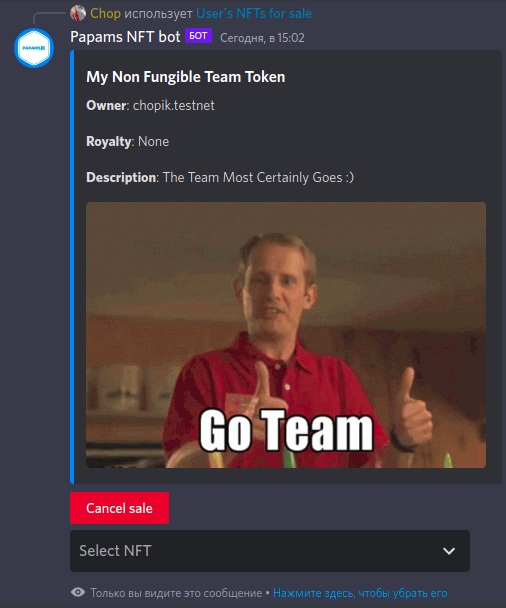
\includegraphics[height=60mm]{fig/mynftonsale.png}
    }
    \subfloat[Общий список NFT пользователя]{
        \label{fig.mynftlistonsale}
        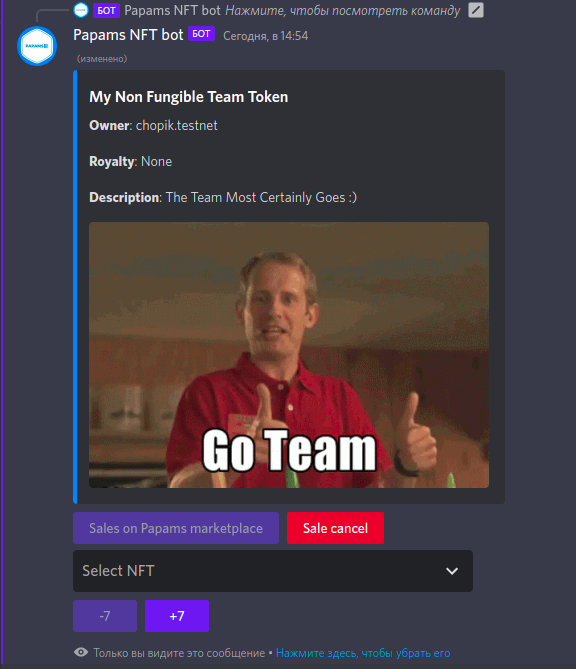
\includegraphics[height=60mm]{fig/mynftlistonsale.png}
    }
    \subfloat[Подтверждение отмены продажи]{
        \label{fig.cancelsaleconfirm}
        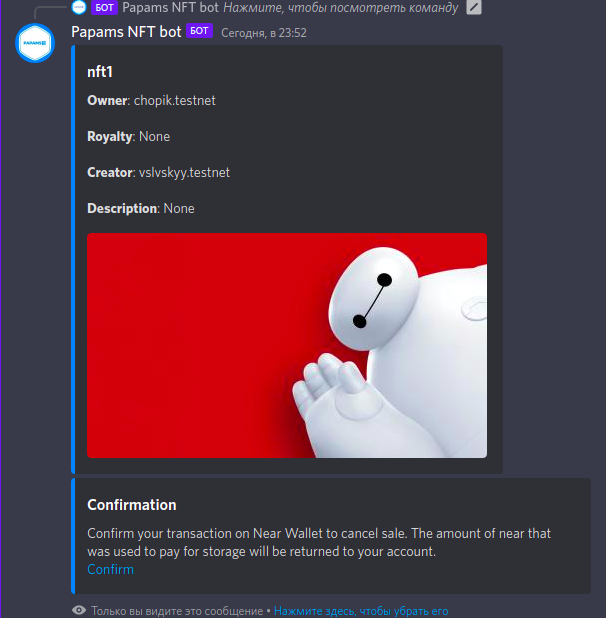
\includegraphics[height=60mm]{fig/cancelsaleconfirm.png}
    }
    \caption{Отмена продажи}
\end{figure}

\begin{remark}
    Визуальный вид списка NFT(Рисунок {\color{blue} \ref{fig.cancelsalenftforsale}}, Рисунок {\color{blue} \ref{fig.mynftlistonsale}}) меняется от их количества: если NFT меньше 7, то не будет кнопок <<+7>>, <<-7>>, которые будут подгружать следующие/предыдущие 7 NFT. Это сделано для того, чтобы в один момент не подгружать все NFT с блокчейна.

\end{remark}

// Лущ Иван. Здесь еще будет про смену цены


\subsection{Деплой бота}
	Чтобы развернуть наш проект в интернете используется Alibaba cloud ecs(Elastic Compute Service). Для деплоя используется проксирование с помощью nginx(Рисунок {\color{blue} \ref{fig.nginxganservice}}).
	\begin{figure}[H]
		\centering
		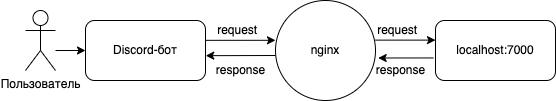
\includegraphics[height=40mm]{fig/nginxganservice.png}
		\caption{Схема деплоя бота}
        \label{fig.nginxganservice}
	\end{figure}

\section{Генеративно-состязательная сеть}
\label{section.6}
// Текст будет написан Токкожиным Арсеном
\section{Сервис с генеративно-состязательной сетью}
\label{section.ganservice}
  В данной главе будет описываться сервис для создания NFT с помощью генеративно-состязательной сети и описание его конракта.
\subsection{Устройство сервиса}

	Сервис представляет собой http-сервис, которому на вход подается GET-запрос от discord-бота и он на своей стороне генерирует картинку, характеристики к ней и формирует URL транзакции.

	Архитектура взаимодейсвия бота и сервера проиллюстрирована на рисунке {\color{blue} \ref{fig.ganservice}}
	\begin{figure}[H]
		\centering
		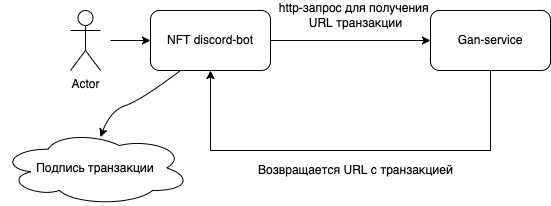
\includegraphics[height=50mm]{fig/gan-service.png}
		\caption{Marketplace contract sell}
		\label{fig.ganservice}
	\end{figure}


\begin{remark}
	Создание нового NFT удовлетворяет следующиму свойству: Пользователь при генерации NFT увидит саму картинку только подписания транзакции
\end{remark}

\subsection{Устройство случайного получения NFT}
 Для того чтобы пользователь не видел картинку которую получит до подписания транзакции мы используем следующую схему:
  Формируем конракт в котором будут N сгенерированых NFT, которые хранятся в динамическом массиве, в этот массив добавляется (N + 1)'ый NFT, но при этом пользователю будет возвращаться случайный NFT из этого массива.
  Таким образом пользователь не сможет угадать, какая именно nft ему выпадет.

            % Основная часть
\section{Результаты и дальнейшие планы}
\label{section.output}
В результате выполнения данной работы были реализованы smart-контракты NFT (по стандарту NEP-171) и маркетплейса, реализован discord-бот, который предоставляет удобный интерфейс пользователю и выполняет роль NFT маркетплейса с функционалом, который планировался изначально, а также реализован сервис для генерации NFT, доступ к которому, пользователь получает через discord-бот.

В качестве дальнейшей работы планируется пересмотр текущего распределенного хранилища, в котором хранятся метаданные и медиа-файл NFT; исправление выявленных багов в discord-боте; добавление нового функционала:
\begin{enumerate}
    \item Создание и привязка токена к коллекциям аналогично paras. В процессе разработки было обнаружено, что такая структура является наиболее удобной, поэтому в будущем данная идея будет позаимствована у paras.
    \item Агрегация токенов по убыванию/возрастанию цены, времени создания, редкости (в случае токенов генерируемыми генеративными моделями).
    \item Возможность сделать оффер (предложение о покупке) на любой токен(как продаваемый, так и не продаваемый). Это очень удобно, например, когда пользователю цена кажется слишком большой и он решает предложить цену меньше, или когда токен не продается и пользователь большой ценой хочет его выкупить.
    \item Сбор статистики о количестве созданных/уничтоженных токенов, объеме продаж за день/месяц/год, количестве сделок за день/месяц/год. Вышеописанную статистику можно собирать также и по конкретному пользователю.
    \item Добавление большего числа генеративных моделей.
\end{enumerate}

\newpage
    % Заключение

\printbibliography[heading=bibintoc]
\newpage

% \section{Приложения}

\subsection{Ссылка на репозиторий}

Ссылка на Gitlab репозиторий с проектом - \href{https://gitlab.com/Ch0p1k3/papams-nft-discord-bot}{\textcolor{blue}{Gitlab}}.
     % Приложения

\end{document}
